% \iffalse meta-comment
%
% Copyright (C) \the\year by Liu Benyuan <liubenyuan@gmail.com>
% This file may be distributed and/or modified under the
% conditions of the LaTeX Project Public License, either
% version 1.2 of this license or (at your option) any later
% version. The latest version of this license is in:
%
% http://www.latex-project.org/lppl.txt
%
% and version 1.2 or later is part of all distributions of
% LaTeX version 1999/12/01 or later.
%
% \fi
% 
% \iffalse
% <package>\NeedsTeXFormat{LaTeX2e}[1999/12/01]
% <package>\ProvidesPackage{nudtpaper}
% <package>		[2009/08/12 v1.0 By Liu Benyuan <liubenyuan@gmail.com>]
%<*driver>
\ProvidesFile{nudtpaper.dtx}[2009/08/12 v1.0 NUDT]
\documentclass[11pt]{ltxdoc}
\usepackage{nudtx}
\EnableCrossrefs
\CodelineIndex
\RecordChanges
\begin{document}
  \DocInput{\jobname.dtx}
\end{document}
%</driver>
% \fi
% 
% \def\thuthesis{\textsc{Thu}\-\textsc{Thesis}}
% \def\nudtpaper{\textsc{Nudt}\-\textsc{Paper}}
% 
% \CheckSum{1224}
% \CharacterTable
%  {Upper-case    \A\B\C\D\E\F\G\H\I\J\K\L\M\N\O\P\Q\R\S\T\U\V\W\X\Y\Z
%   Lower-case    \a\b\c\d\e\f\g\h\i\j\k\l\m\n\o\p\q\r\s\t\u\v\w\x\y\z
%   Digits        \0\1\2\3\4\5\6\7\8\9
%   Exclamation   \!     Double quote  \"     Hash (number) \#
%   Dollar        \$     Percent       \%     Ampersand     \&
%   Acute accent  \'     Left paren    \(     Right paren   \)
%   Asterisk      \*     Plus          \+     Comma         \,
%   Minus         \-     Point         \.     Solidus       \/
%   Colon         \:     Semicolon     \;     Less than     \<
%   Equals        \=     Greater than  \>     Question mark \?
%   Commercial at \@     Left bracket  \[     Backslash     \\
%   Right bracket \]     Circumflex    \^     Underscore    \_
%   Grave accent  \`     Left brace    \{     Vertical bar  \|
%   Right brace   \}     Tilde         \~}
%
% \changes{v0.99}{2009/08/12}{Initial Release}
%
% \GetFileInfo{\jobname.dtx}
% 
% \DoNotIndex{\begin,\end,\begingroup,\endgroup}
% \DoNotIndex{\ifx,\ifdim,\ifnum,\ifcase,\else,\or,\fi}
% \DoNotIndex{\let,\def,\xdef,\newcommand,\renewcommand}
% \DoNotIndex{\expandafter,\csname,\endcsname,\relax,\protect}
% \DoNotIndex{\Huge,\huge,\LARGE,\Large,\large,\normalsize}
% \DoNotIndex{\small,\footnotesize,\scriptsize,\tiny}
% \DoNotIndex{\normalfont,\bfseries,\slshape,\interlinepenalty}
% \DoNotIndex{\hfil,\par,\hskip,\vskip,\vspace,\quad}
% \DoNotIndex{\centering,\raggedright}
% \DoNotIndex{\c@secnumdepth,\@startsection,\@setfontsize}
% \DoNotIndex{\ ,\@plus,\@minus,\p@,\z@,\@m,\@M,\@ne,\m@ne}
% \DoNotIndex{\@@par,\DeclareOperation,\RequirePackage,\LoadClass}
% \DoNotIndex{\AtBeginDocument,\AtEndDocument}
%
% \IndexPrologue{\section*{索引}%
%    \addcontentsline{toc}{section}{索~~~~引}}
% \GlossaryPrologue{\section*{修改记录}%
%    \addcontentsline{toc}{section}{修改记录}}
%
% \renewcommand{\abstractname}{摘~~要}
% \renewcommand{\contentsname}{目~~录}
%
% \title{\textsc{NUDTpaper:}\,\,NUDT研究生学位论文\LaTeX{}模板使用手册\thanks{NUDT \LaTeX{} Thesis Template}}
% \author{刘本源 \\ \texttt{Liubenyuan@gmail.com}}
% \date{\fileversion\ (\filedate)}
%
% \maketitle
% \thispagestyle{empty}
%
% \begin{abstract}
% 本模板旨在提供规范的国防科学技术大学\LaTeX{}写作模板环境,
% 现支持硕士/博士学位论文格式,可以自动生成盲评、制作A3封面。
% \end{abstract}
%
% \vspace{2cm}
% \def\abstractname{免责声明}
% \begin{abstract}\noindent
% \begin{enumerate}
% \item 本模板的发布遵守 \LaTeX{} Project Public License,使用前请认真阅读协议内容
% \item 本模板创立参照官方严格的论文写作手册,并同时参照硕士/博士学位论文\textbf{doc}文档对比修改
% \item 国防科学技术大学对论文写作提供写作指南与官方\textbf{doc}模板,
% 同时提供官方的\LaTeX{}模板,本模板的出发点是方便大家使用专业的高效的论文书写工具,
% 其有点在于注重排版质量、命令规范、使用方便、更新及时,符合论文撰写说明。
% 但任何由于使用本模板而引起的论文格式审查问题均与本模板作者无关。
% \item 任何个人或组织均可以本模板为基础进行修改、扩展,生成新的专用模板,但请严格遵
% 守\LaTeX{} Project Public License 协议
% \item 欢迎提出修改意见
% \end{enumerate}
% \end{abstract}
%
% \clearpage
% \tableofcontents
%
% \clearpage
% \pagenumbering{arabic}
% \pagestyle{mainpage}
%
% \section{快速上手}
% 这部分是专门为那些想快速开始写论文的人准备的。
% \begin{description}
% \item[安装\TeX] 下载最新的\TeX{}live或者C\TeX{}并安装
% \item[字体] 用户需要具备\verb|simsun.ttf|, \verb|simhei.ttf|, \verb|simkai.ttf|,
% \verb|STZHONGS.TTF|, 上述字体都是windows自带的; 除此之外,在网上搜索(或者C\TeX{}
% 论坛)``Adobe Opentype 中文字体'',一搜一大把,确保下载下来Adobe的四款OTF字体:
% 宋,黑,仿宋,楷体。Linux用户可将上述字体复制到\verb|/usr/share/fonts/TTF|下。
% \item[试一试] 解压缩下载的模板,双击makepdf.bat(祈祷一下),如果生成了
% \verb|thesis.pdf|$\rightarrow$
% \item[那么我的那些常用的包都在么?] 你会想我的{\bf Trans}论文可以无缝
% 的复制过来么? 对于这一点,你可以修改\verb|mynudt.sty|来实现。但是{\hei 注意},大部分包
% 都在模板中了,而且{\hei 切记切记},不要擅自改动字体等版面设计,我们继续看$\rightarrow$
% \item[咦,数学公式不是很美观呀] 笔者{\hei 强烈}建议用户使用{\bf mtpro2}宏包的,怎么使用,
% 又有哪些好处,参见bookzh.sty吧!不会错的。好了,我们专注于内容本身吧$\rightarrow$
% \item[开始写了] 所有文件均采用UTF8编码,因此要保证你的\TeX{}编辑器
% (winedt, texworks, texmaker, vim, 记事本($\cdots{}$)等)支持这种编码,
% (经过一番搜索设置后)打开\verb|thesis.tex|,如果看到的是中文$\rightarrow$
% \item[漫长的写作] 手边准备着\LaTeX{}的常用帮助文档(数学,图表,引用等),
% 结合你喜欢的文献管理软件(JabRef等), 漫长的\texttt{编辑,编译,修改,编辑,
% 编译$\cdots$}过程之后,突然有一天发现你写完了$\rightarrow$
% \item[校订] 经过老师师兄师弟师妹齐心协力校正之后,你所做的只是:
% \texttt{生成明评论文,制作明评封面,生成盲评论文,制作盲评封面},
% 装订,上交$\rightarrow$
% \end{description}
% {\color{magenta} Done!}
%
% \section{模板介绍}
%
% \textsc{NUDTpaper} 旨在帮助并且推广\LaTeX{}在国防科技大学论文中的应用,
% 本文将尽可能帮助用户掌握\textsc{NUDTpaper}的安装方法,
% 如果仍旧有不清晰的地方可以参考样例文件或者
% 给作者邮件\footnote{liubenyuan@gmail.com},感兴趣的同学可以帮忙维护模板,
% 这个模板首先符合官方的设计要求,希望同学们在使用后能够提出你们的修改意见。
% 该模板很大程度上参考了6院黄老师sofoot的国防科大博士论文模板,
% 哈工大的\LaTeX{}模板以及清华的Thuthesis
% \footnote{主页:\url{http://thuthesis.sourceforge.net}},
% 有很多使用的帮助、\verb|.cls|中的命令以及版面设置均来自Thuthesis和sofoot的模板,
% 对此的引用表示感谢。
%
% {\color{blue}\fs 模板的作用在于减轻论文写作过程中格式调整的时间,
% 其前提就是遵守模板的用法,不提倡手动更改格式,不建议正文中使用
% 手动调节版面的命令,尤其禁止修改行距和使用\verb|\normalsize|,
% 否则即使使用了\textsc{NUDTpaper}也难以保证输出的论文符合学校规范。}
%
% \section{安装}
% \label{sec:install}
%
% \subsection{下载}
% \textsc{NUDTpaper} 主页:\url{http://nudtpaper.googlecode.com}。
% 模板的更新信息发布在\href{http://bbs.ctex.org}{Ctex论坛}。
% \nudtpaper{}的开发版本同样可以在\textsc{gitorious}上获得。
%
% \subsection{模板的组成部分}
% 下表列出了 \nudtpaper{} 的主要文件及其功能介绍,学习模板的最好办法
% 就是参考thesis.pdf!
% \begin{center}
% \begin{longtable}{l|p{8cm}}
% \toprule
% {\hei 文件(夹)} & {\hei 功能描述}\\\midrule
% \endfirsthead
% \toprule
% {\hei 文件(夹)} & {\hei 功能描述}\\\midrule
% \endhead
% \endfoot
% \endlastfoot
% nudtpaper.ins & 模板驱动文件 \\
% nudtpaper.dtx & 模板文档代码的混合文件\\
% nudtpaper.cls & 模板类文件\\
% nudtpaper.cfg & 模板配置文件\\
% thesis.bib & 参考文献样式文件\\
% \hline
% mynudt.sty & 在这里添加你自己的宏包 \\
% thesis.tex & 示例文档主文件\\
% ref/ & 示例文档参考文献目录\\
% data/ & 示例文档章节具体内容\\
% figures/ & 示例文档图片路径\\
% \textbf{nudtpaper.pdf} & 用户手册(本文档)\\
% \textbf{thesis.pdf} & 示例文档 \\
% \bottomrule
% \end{longtable}
% \end{center}
%
% \subsection{\TeX{}系统的选择}
% 有网络环境的用户推荐安装\href{http://www.tug.org/texlive}{\TeX{}live},
% \href{http://miktex.org}{MiKTeX}或者\href{http://www.ctex.org}{C\TeX},
% 对于无网络环境的,主要是针对教研室用户,推荐{\TeX{}live}或者C\TeX{}完整版,安装
% 过程很简单,一路下一步即可,但是需要\textbf{注意:}
%
% \begin{description}
% \item[字体] TTF选项默认调用Windows系统字体,其中楷体、仿宋需要安装Office;OTF选项需要
% Adobe的商业字体(可以使你的论文更加漂亮!),这些中文字体(宋,黑,仿宋,楷体)可以从
% \href{http://dl.getdropbox.com/u/857066/adobe_chinese_otf.7z}{这里下载},
% 如果上述链接不能使用,请搜索\textsc{Adobe Opentype 中文字体}自行下载。
% 英文字体使用Windows自带。起始更推荐几款Times(Arial)类似的OTF英文字体,可以使用
% 更多排版、段落的字体特性。
% \item[粗宋] 模板中在需要宋体加黑的地方需要使用\textbf{华文中宋}, 即STZHONGS.TTF。
% \item[xeCJK] 无网络环境中,C\TeX{}完整版和\TeX{}live最新版都包括了需要的xeCJK版本。
% \end{description}
%
% \subsection{使用模板}
% \label{sec:install-cls}
% {\hei 注:默认的发行版本已经包含了可以使用的模板环境,
% 包括编译好的cls以及论文样例源文件,
% 想快速上手的话,可以直接参看\verb|thesis.tex|,进行修改。
% 写作的过程就是将你的论文的内容放到\verb|data|文件夹中,
% 图片放到\verb|figures|文件夹中,用\textsc{jabref}修改\verb|thesis.bib|即可。}
%
% 当用户需要编译生成自己的PDF版论文时,需要依次输入:(注意了,如果不是使用nomencl,
% 则无需使用第二个命令)
% \begin{shell}
% $ xelatex thesis
% $ # makeindex -s nomencl.ist -o thesis.nls thesis.nlo
% $ bibtex thesis
% $ bibtex thesis
% $ xelatex thesis
% $ xelatex thesis
% \end{shell}
%
% 而为了简化用户使用,模板中提供了快捷脚本文件:
% \begin{shell}
% # 下面命令可以直接生成thesis.pdf,你可能只需要这步
% C:\> makepdf.bat
% # linux用户可以直接使用makefile
% $ make pdf
% \end{shell}
% 现在,就要进入激动人心的写作过程了。
%
% \section{使用说明}
% \label{sec:how-to-use}
% 首先,一篇论文(电子信息工程专业为例),主要的构成就是
% 封面导言,正文,表格,图片,公式,
% 交叉引用及文献索引这五部分,下面将分别详细讲解。
%
% \label{sec:howtoask}
% 在开始之前,先问自己几个问题:
% \begin{compactenum}
% \item 我是不是已经掌握了 \LaTeX{} 基础知识?
% \item 我是不是认真地阅读了模板文档?
% \item 周围有没有同学可以帮我?
% \end{compactenum}
% 更推荐用户去阅读示例文档的源代码,改写会给你一个快速的开始。
%
% \subsection{示例文件}
% \label{sec:example}
% 该示例文件是顶层的文件,包括论文属性设置、章节的安排、参考文献附录等。
% 细节用户可以参考\verb|thesis.tex|和\verb|data/|文件夹。
%
% \subsubsection{模板选项}
%
% 论文的第一句话是调用模板:
% \changes{v2.0}{2010/11/10}{增加盲评的说明}
%
%    \begin{macrocode}
%<thesis>%1. 规范硕士导言
%<thesis>% \documentclass[master,ttf]{nudtpaper}
%<thesis>%2. 规范博士导言
%<thesis>% \documentclass[doctor,twoside,ttf]{nudtpaper}
%<thesis>%3. 如果使用是Vista
%<thesis>% \documentclass[master,ttf,vista]{nudtpaper}
%<thesis>%4. 建议使用OTF字体获得较好的页面显示效果
%<thesis>%   OTF字体从网上获得,各个系统名称统一,不用加vista选项
%<thesis>%   如果你下载的是最新的(1201)OTF英文字体,建议修改nudtpaper.cls,使用
%<thesis>%   Times New Roman PS Std
%<thesis>% \documentclass[doctor,twoside,otf]{nudtpaper}
%<thesis>%   另外,新版的论文模板提供了方正字体选项FZ,效果也不错哦
%<thesis>% \documentclass[doctor,twoside,fz]{nudtpaper}
%<thesis>%5. 如果想生成盲评,传递anon即可,仍需修改个人成果部分
%<thesis>% \documentclass[master,otf,anon]{nudtpaper}
%<thesis>%
%    \end{macrocode}
%    \begin{macrocode}
%<*thesis>
\documentclass[master,otf]{nudtpaper}
\usepackage{mynudt}

%</thesis>
%    \end{macrocode}
%
% 模板的参数设置(开关)描述见:
%
%\begin{description}
%\item[master,doctor]
% 硕士论文用master,博士论文就用doctor
%\item[twoside]
% 指定论文为单面打印还是双面打印,当使用\verb|twoside|选项之后,
% 论文会将章节开在奇数页右手边,默认为\verb|openany|单面打印。
%\item[ttf,otf]
% 决定使用何种字体,TTF默认使用Windows自带的字体,而OTF则使用Adobe的字体(需要下载),
% TTF字体的优势是满足学校论文对于字体的要求,缺点是制作出来的PDF文件在浏览时可能发虚,
% 而OTF字体屏幕显示饱满,而且字体有很多选项可以方便\XeTeX{}排版。推荐使用\textbf{otf}
% 选项。不论何种选项,都需要安装宋体中宋(STZHONGSONG)字体(Windows自带)。
%\item[vista]
% 使用\textsc{vista}的用户当调用模板的TTF字体时,系统默认的楷体、仿宋名称是KaiTi和FangSong,
% 而不是KaiTi\_GB2312,这里加入开关进行切换。
%\item[anon]
% 是否为盲评版本,如需盲评,请加上anon。
%\end{description}
%
% 如果需要使用自己定义的命令、宏包,请放于\verb|mynudt.sty|中。
% 事实上,该文件中已经添加了很多有用的宏包和命令,你可以参照修改。
% 这些之所以没有放到模板中,一则为了简洁,二则赋予用户在格式之外更多的自由。
% 里面的宏包有:代码高亮、算法环境、向量命令等,请仔细查看。
%
% 样例文件默认的是硕士论文(master),OTF字体(otf)。
%
% \subsubsection{封面导言}
% 官方模板中设计论文题目、作者等信息可以跟填空一样完成:
%
% \begin{description}
% \item[论文封头]
% 主要有四部分内容,中图分类号,学号,论文密级和UDC。
% 密级分为:\textbf{秘密} 或者 \textbf{公开}。
%    \begin{macrocode}
%<*thesis>
\classification{TP957}
\serialno{0123456}
\confidentiality{公开}
\UDC{}
%</thesis>
%    \end{macrocode}
%
% \item[论文题目,作者,日期]
% 分别包括中文和英文两部分,由于论文题目可能超过1行,
% 我们提供额外的一个命令\verb|\displaytitle|用来在
% 授权书中填入(限定为)单行的题目; 中文日期需要中文输入大写,英文日期为月年,
% 在论文最终完成后,请\textbf{手动}设定日期。
%
%    \begin{macrocode}
%<*thesis>
\title{国防科大学位论文\LaTeX{}模板\\
使用手册}
\displaytitle{国防科学技术大学学位论文\LaTeX{}模板}
\author{张三}
\zhdate{\zhtoday}
\entitle{How to Use the \LaTeX{} Document Class for NUDT Dissertations}
\enauthor{Zhang San}
\endate{\entoday}
%</thesis>
%    \end{macrocode}
%
% \item[论文分类及其他]
% 主要是作者的学科类别,研究方向,导师信息等。
% 每一项都包括中英文信息:
%
%    \begin{macrocode}
%<*thesis>
\subject{通信与信息工程}
\ensubject{Information and Communication Engineering}
\researchfield{自动目标识别与模糊工程}
\supervisor{李四\quad{}教授}
\cosupervisor{王五\quad{}副教授} % 没有就空着
\ensupervisor{Professor Li Si}
\encosupervisor{}
\papertype{工学}
\enpapertype{Engineering}
%</thesis>
%    \end{macrocode}
%
% \item[中英文摘要]
% 论文中需要写中文以及英文摘要,页码为小写罗马字母,关键字为黑体,
% 英文关键字为\verb|Arial|,
% 模板中定义了相关环境\verb|\cabstract|以及\verb|\eabstract|来书写摘要,
% 以及\verb|\ckeywords|以及\verb|\ekeywords|来写关键字。
% 建议用户将摘要单独放在在\verb|abstract.tex|文件中,
% 在正文中\verb|\begin{cabstract}
国防科学技术大学是一所直属中央军委的综合性大学。1984年,学校经国务院、中央军委和教育部批准首批成立研究生院,%
肩负着为全军培养高级科学和工程技术人才与指挥人才,培训高级领导干部,从事先进武器装备和国防关键技术研究的重要任务。%
国防科技大学是全国重点大学,也是全国首批进入国家“211工程” 建设并获中央专项经费支持的全国重点院校之一。%
学校前身是1953年创建于哈尔滨的中国人民解放军军事工程学院,简称“哈军工”。
\end{cabstract}
\ckeywords{国防科学技术大学; 211; 哈军工}

\begin{eabstract}
National University of Defense Technology is a comprehensive national key university based in Changsha, %
Hunan Province, China. It is under the dual supervision of the Ministry of National Defense %
and the Ministry of Education, designated for Project 211 and Project 985, %
the two national plans for facilitating the development of Chinese higher education. %

NUDT was originally founded in 1953 as the Military Academy of Engineering in Harbin of Heilongjiang Province. %
In 1970 the Academy of Engineering moved southwards to Changsha and was renamed Changsha Institute of Technology.%
 The Institute changed its name to National University of Defense Technology in 1978.

\end{eabstract}
\ekeywords{NUDT; MND; ME}

|即可。其格式为:
%
% \begin{example}
% \begin{cabstract}
% 中文摘要
% \end{cabstract}
% \ckeywords{关键字}
%
% \begin{eabstract}
% Abstract
% \end{eabstract}
% \ekeywords{Key}
% \end{example}
% \end{description}
%
% \subsubsection{框架构成}
%
% 在定义完论文元素之后,就可以开始写论文正文了。用\LaTeX{}写论文的文件目录构成
% 可以很随意,模板中将图形文件单独放到一个目录中\verb|figure|中,论文正文各个
% 章节置于\verb|data|中;当然也以以\verb|chapter|为目录。
%\changes{v2.2}{2011/05/27}{使用nomencl包管理符号列表}
%\changes{v2.2}{2011/07/08}{默认使用nomencl管理参考文献}
%\changes{v2.2}{2011/09/10}{回复原先使用的denotation方式添加符号列表}
% 
% 如果使用nomencl制作符号列表,在文档开始前要加入\verb|\makenomenclature|命令
% 默认还是使用denotation的方式。nomencl可以参考第二章相关章节,而denote方式
% 请参考\verb|data/denotation.tex|文件(简单的列表环境)。
% 
%<thesis>% 加入makenomenclature命令可用nomencl制作符号列表。
%
%    \begin{macrocode}
%<*thesis> 

\begin{document}
\graphicspath{{figures/}}
%</thesis>
%    \end{macrocode}
% 制作完封面后就是正文四大部分了,分别为:
%
% \begin{compactenum}
% \item frontmatter: 生成目录,图目录,表目录
% \item midmatter: 摘要,符号列表
% \item mainmatter: 正文,致谢,文献,成果
% \item backmatter: 附录
% \end{compactenum}
%
%<thesis>% 制作封面,生成目录,插入摘要,插入符号列表 \\
%<thesis>% 默认符号列表使用denotation.tex,如果要使用nomencl \\
%<thesis>% 需要注释掉denotation,并取消下面两个命令的注释。 \\
%<thesis>% cleardoublepage% \\
%<thesis>% printnomenclature% \\
%
%    \begin{macrocode}
%<*thesis>
\maketitle
\frontmatter
\tableofcontents
\listoftables
\listoffigures

\midmatter
\begin{cabstract}
国防科学技术大学是一所直属中央军委的综合性大学。1984年,学校经国务院、中央军委和教育部批准首批成立研究生院,%
肩负着为全军培养高级科学和工程技术人才与指挥人才,培训高级领导干部,从事先进武器装备和国防关键技术研究的重要任务。%
国防科技大学是全国重点大学,也是全国首批进入国家“211工程” 建设并获中央专项经费支持的全国重点院校之一。%
学校前身是1953年创建于哈尔滨的中国人民解放军军事工程学院,简称“哈军工”。
\end{cabstract}
\ckeywords{国防科学技术大学; 211; 哈军工}

\begin{eabstract}
National University of Defense Technology is a comprehensive national key university based in Changsha, %
Hunan Province, China. It is under the dual supervision of the Ministry of National Defense %
and the Ministry of Education, designated for Project 211 and Project 985, %
the two national plans for facilitating the development of Chinese higher education. %

NUDT was originally founded in 1953 as the Military Academy of Engineering in Harbin of Heilongjiang Province. %
In 1970 the Academy of Engineering moved southwards to Changsha and was renamed Changsha Institute of Technology.%
 The Institute changed its name to National University of Defense Technology in 1978.

\end{eabstract}
\ekeywords{NUDT; MND; ME}


\chapter*{符号使用说明}
% 可以根据需要在chapter后加星星/去掉星星

\begin{denotation}

\item[HPC] 高性能计算 (High Performance Computing)
\item[cluster] 集群
\item[Itanium] 安腾
\item[SMP] 对称多处理
\item[API] 应用程序编程接口
\item[PI]	聚酰亚胺
\item[MPI]	聚酰亚胺模型化合物,N-苯基邻苯酰亚胺
\item[PBI]	聚苯并咪唑
\item[MPBI]	聚苯并咪唑模型化合物,N-苯基苯并咪唑
\item[PY]	聚吡咙
\item[PMDA-BDA]	均苯四酸二酐与联苯四胺合成的聚吡咙薄膜
\item[$\Delta G$]  	活化自由能~(Activation Free Energy)
\item [$\chi$] 传输系数~(Transmission Coefficient)
\item[$E$] 能量
\item[$m$] 质量
\item[$c$] 光速
\item[$P$] 概率
\item[$T$] 时间
\item[$v$] 速度

\end{denotation}


%</thesis>
%    \end{macrocode}
%
%<thesis>%书写正文,可以根据需要增添章节; 正文还包括致谢,参考文献与成果
%\changes{v1.4}{2009/10/31}{将成果移动到参考文献之后}
%
%    \begin{macrocode}
%<*thesis>
\mainmatter
\chapter{绪论}
本章首先对本文研究的课题背景和研究意义进行介绍,然后对本文的研究内容和文章的
组织结构予以说明。
\section{本文研究背景和意义}
规模化传感网既是前沿研究问题,又在国家社会重大安全领域有着预期的应用前景,预期将得到广泛应用和持续的发展。本研究适应大规模大数据无线传感需求的数据认证机制,设计相关认证算法、协议及有关密钥分配管理的算法,并将在仿真平台和实际传感器节点平台上实现、验证和测试有关功能。将为大规模大数据无线传感网的数据认证提供可行的技术方案,为了解决无线传感网的安全传输提供了工程上的解决范例。



\subsection{无线传感网概述}
正文内容

正文内容


\subsection{无线传感网对数据认证的需求}
无线传感网的安全需求主要有两方面:面向基础设施的通信安全及面向数据的信
息安全。前者为无线传感网完成数据采集、数据传输、数据融合等基本功能提供支
撑,后者提供实现数据机密性、完整性、不可否认性等信息安全机制。
通信安全主要包括以下内容:
- 节点安全性:指传感器节点的部署隐蔽性及抗受损能力。要求节点不易被发现,
且节点内部通过代码混淆等方法提供一定的机密信息保护措施。
- 防御能力:指无线传感网抗外部攻击及内部攻击的能力。要求在敌手攻击下,部
分节点受损不会影响网络的整体功能。
- 入侵检测能力:指识别入侵行为,确定入侵者身份、位置等信息,主动丢弃入侵
者发出的虚假数据的能力。

信息安全主要包括以下内容:
- 数据机密性:通过加密技术及访问控制能确保网络中的消息明文不会暴露给非授
权实体。
- 不可否认性:通过消息签名、身份认证、访问控制等方式有效识别消息源。
- 数据完整性:通过消息认证码(MAC)、消息签名等技术提供数据在传输过程中的
防篡改能力。
- 数据新鲜性:通过消息新鲜性参数确保消息在其时效范围内被目标实体接收。


除了保证必要的通信安全及数据安全,安全协议的设计还应当考虑如下因素:
- 抗毁性:部分节点受损不会导致整个网络安全体系瘫痪。
- 可扩展性:安全协议不应当对网络节点的加入与移除造成影响。
- 灵活性:安全协议不应当影响网络部署的灵活性。
- 低开销:安全协议带来的计算开销、通信开销、存储开销及对应能耗应当是传感
器节点可承受的。

\section{本文研究内容}
正文内容

正文内容

正文内容

正文内容

\section{本文组织结构}



\chapter{相关研究概述}
无线传感网在环境监测、工业控制、资源监测和军事侦察等领域都有重要的应用,具有非常良好的前景。但是区别于传统的网络,无线传感器节点一般都部署在无人值守的环境恶劣地区或敌对区域,可能受到敌人的攻击破坏,所以安全问题十分突出。同时由于无线传感器节点的存储空间和计算能力的限制,安全机制的复杂性受到约束,因此设计适合无线传感网应用需求的安全机制十分重要。

本章首先对无线传感网的安全技术进行概述,然后对无线传感网的认证机制及其密钥分配方案进行概述。

\section{无线传感网安全技术概述}
无线传感网的节点一般部署在无人值守区域,使得无线传感网的安全问题尤为突出,特别是在军事侦察等应用领域。无线传感网不能直接沿用传统无线网络的安全机制,设计无线传感网的安全机制时,必须考虑到无线传感器网的如下限制
\upcite{c1:limitation}:
\begin{compactitem}
  \item 节点的存储空间、计算能力和通信能力有限,特别是节点的能量有限,严重制约了安全机制的发展。
  \item 无线传感网有无线自组网的缺点,缺乏基础设施建设,节点之间使用不安全的无线通信。
  \item 部署的位置一般是敌对区域或者危险区域,节点很容易受到物理攻击或者破坏。
\end{compactitem}

无线传感网的应用决定了其安全目标与传统网络有所不同,更侧重于保护感知的数据,保证数据的安全。
在无线传感网中,安全技术的目标主要包括\upcite{c1:attack}:
\begin{compactitem}
  \item 数据认证:通过认证确保数据来自经过身份认证的节点,保证数据的安全。
  \item 数据保密:确保只有通过认证的节点才能获取消息中的内容,不会暴露保密的内容。
  \item 数据完整性:确保所有受到的消息没有被未经授权的设备所篡改。
  \item 可用性:确保传感器节点在受到攻击时仍然能提供指定的基本服务。
  \item 数据新鲜:保证数据在指定时间内到达目的节点,确保数据的有效性。
\end{compactitem}

\subsection{无线传感网面临的安全威胁}

无线传感网的协议栈包括传输层、网络层、链路层和物理层,各层都会遭到不同的攻击。对于各层的攻击,有各种防御手段来保护无线传感网的安全,传输层主要研究认证机制及面向认证的密钥管理技术,网络层主要研究路由安全协议,数据链路层主要研究数据帧的安全传输,物理层主要研究节点间通信信道安全。
无线传感网中常见的攻击与防御措施\upcite{c1:attack}如表~\ref{tb:wsnattack}所示:

\begin{table}[htbp]
  \centering
  \caption{无线传感网常见的攻击与防御措施}
  \label{tb:wsnattack}
  \begin{minipage}[t]{0.8\textwidth}
    \begin{tabularx}{\linewidth}{|c|c|X|}
      \hline
%      \multirow{1}*{网络层次}
%        & 常见的攻击 & 防范措施\\
      \multirow{1}*{网络层次}  & \multicolumn{1}{c|}{常见的攻击} & \multicolumn{1}{c|}{防范措施}\\
      \hline
      \multirow{2}*{传输层}
        & 泛洪攻击 & 用户询问 \\\cline{2-3}
        & 同步破坏攻击 & 认证机制 \\
      \hline
      \multirow{7}*{网络层}
        & 泛洪攻击 & 广播和组播半径限制 \\\cline{2-3}
        & 黑洞攻击 & 节点身份认证,冗余路径 \\\cline{2-3}
        & 错误定向攻击 & 数据帧转发签名 \\\cline{2-3}
        & 蠕虫洞攻击 & 基于信任等级的路由 \\\cline{2-3}
        & 创建路由环 & 篡改校验、认证 \\\cline{2-3}
        & 汇聚节点攻击 & 加密、逐跳认证机制 \\\cline{2-3}
        & 虚假路由攻击 & 冗余机制、数据一致性检测 \\
      \hline
      \multirow{3}*{数据链路层}
        & 资源耗尽攻击 & 限制通信速度,竞争门限控制 \\\cline{2-3}
        & 碰撞攻击 & 纠错校验码 \\\cline{2-3}
        & 非公平竞争攻击 & 使用非优先级策略 \\
      \hline
      \multirow{3}*{物理层}
        & 拥塞攻击 & 使用优先级消息、宽频通信、间歇通信 \\\cline{2-3}
        & 无线干扰 & 变频通信、跳频通信 \\\cline{2-3}
        & 物理破坏 & 节点伪装和隐藏 \\
      \hline
    \end{tabularx}\\[2pt]
  \end{minipage}
\end{table}

物理层受到的攻击主要包括拥塞攻击、无线干扰和物理破坏。拥塞攻击是物理层最常见的攻击,Xu 等就提出了4种不同的拥塞攻击方法\upcite{c1:jamming},能够使无线传感网停止工作。无线干扰是干扰传感器节点的通信信道,和拥塞攻击一样都能严重影响节点的数据发送和接收。通过物理攻击,篡改节点信息是物理层的另一种攻击方法,攻击者能获得节点的内存信息,包括密钥和加密数据,从而破坏该节点的工作。

数据链路层容易受到碰撞攻击,攻击者利用协议的漏洞,在无线传感网发送大量的干扰数据包,与正常数据包传输发生碰撞,造成无线传感网正常数据无法传输,并且消耗节点能量。数据链路层还容易受到资源耗尽攻击,即向特定节点发送大量数据,消耗其节点能量,使之失效。非公平竞争是指攻击者通过发送高优先级的数据包,在网络中一直占据通信信道,使得正常节点一直无法使用信道,无法发送数据。

在无线传感网中,大量的传感器节点部署在监测区域内,报文需要经过多跳才能到达基站,无线传感网的特性决定了它没有固定的拓扑结构,所以每个节点都能进行路由,因此攻击者可以利用该特点发动网络层攻击。网络层受到的攻击包括泛洪攻击、黑洞攻击、错误定向攻击、蠕虫洞攻击、创建路由环攻击、汇聚节点攻击和虚假路由攻击。

传输层受到的攻击包括泛洪攻击和同步破坏攻击。当攻击者发送大量的连接请求,就能严重影响到无线传感网的通信,甚至无法进行正常网络通信,也就是泛洪攻击。同步破坏攻击是指向建立了通信连接的节点不断发送伪造的发送失败消息,使节点一直因为帧丢失而进行重传,而且达到攻击传感器网络的目的。

无线传感网各个协议栈都容易受到攻击,虽然都有相应的防御的措施,但是现阶段的安全机制方案还不够完善,严重制约了无线传感网的应用和发展。


\subsection{无线传感网现有的安全技术}

无线传感网面临着多种攻击的威胁,许多安全技术方案在保护其安全方面已经有了突破。
对于无线传感网的安全技术,在保证数据传输安全的前提下,其设计要考虑到如下需求:
\begin{compactitem}
  \item 稳定性:整个无线传感网的安全体系不会因为个别节点的失效或者被攻击而瘫痪。
  \item 可扩展性:传感网加入新节点,不会对原有的安全体系造成影响,同时不应产生过大的计算开销。
  \item 灵活性:安全技术不能影响到网络的部署结构的灵活性。
  \item 低开销:安全技术的计算开销、通信开销和存储开销应当适合无线传感器节点的能力,不会影响到节点的正常功能。
\end{compactitem}


无线传感网现有的安全技术主要包括加密算法、安全路由、数据聚合、入侵检测、认证机制和密钥管理,其中认证机制和密钥管理将在2.2节与2.3节进行详细论述。

\subsubsection{密码算法}
由于无线传感器节点自身的局限性,计算能力和节点存储空间有限,导致目前非对称密码算法在传感器节点不能直接应用。而对称密码算法需要的计算能力更小,存储空间开销也相对较小,因而目前的传感器网络主要使用的是对称密码算法。如RC5\upcite{c1:RC5}、RC6\upcite{c1:RC6}、Camellia\upcite{c1:Camellia}、TEA\upcite{c1:TEA} 和MISTY1\upcite{c1:MISTY1}等对称加密应用在无线传感网中,在文献\cite{c1:encryptionCompare}中,Law等对这些对称加密算法在无线传感器节点中的运行性能进行了比较和分析。

虽然现阶段非对称密码还很少应用在无线传感网的安全协议中,但是随着硬件技术的进步,传感器节点的计算和存储能力不断提高,低开销的非对称密码算法应用在无线传感网的安全协议中成为了可能,也成为了现阶段无线传感网密码算法研究的热点。现阶段非对称密码在传感器节点上的尝试主要是基于椭圆曲线的密码算法(ECC),David等将ECC应用在TinyOS中
\upcite{c1:EC},Gura等将ECC和RSA在MICA上成功实现\upcite{c1:ECC},并对它们进行了分析比较。
\subsubsection{安全路由}
路由技术在传统的网络中有非常成熟的协议,但是由于无线传感网的特性,没有特定的路由节点,每个节点都要完成路由的功能,导致无线传感网的路由技术与传统网络有较大区别。现阶段多数路由协议都注重提高路由效率,以降低节点的能量消耗,但是这样也造成了潜在的安全问题。

许多相关研究都针对无线传感网的路由安全问题进行了探索,如Deepak等提出的多路由机制\upcite{c1:multiroute},通过在多条路径上传输同一个数据报文,来防御选择性转发攻击,但是该方案中,数据报文需要传输多次,造成通信开销的浪费。还有其他路由协议通过加密和认证等方法提高路由的安全性能,如Karlof等人的方案\upcite{c1:Karlof03}和Li等人的方案
\upcite{c1:Li}。
\subsubsection{数据聚合}
数据聚合减少了无线传感网中的冗余数据,降低了通信开销,节约了节点能量。通过数据聚合安全机制,提高了无线传感网中数据私密性,提高了网络传输的安全性。

Priyanka等人在数据聚合中添加了错误数据检测机制,提出了一种高效的数据聚合方案\upcite{c1:Priyanka},保证了数据的安全传输。类似的研究还有Suat等人的方案\upcite{c1:suat},通过将数据聚合和安全传输以及错误报文过滤相结合,提高了无线传感网数据传输的安全。

Sivagami等人提出的方案\upcite{c1:Sivagami} 中,通过多节点对之间延迟发送消息认证码来对发送的数据进行认证,实现了安全的数据聚合,并且降低了传输开销。

Zhu等人提出了一种错误数据报文过滤机制\upcite{c1:zhu},通过节点间的交叉认证,保证了错误报文在被捕获节点不超过设计参数的情况下会在路径中被过滤。

\subsubsection{入侵检测}
当无线传感器节点的部署在敌对区域时,很容易受到攻击,节点被捕获或者受损不可避免,而攻击者可以通过这些妥协节点发送进一步的攻击,从而影响整个无线传感网的安全。因此在无线传感网中,入侵检测技术可以发现网络中的异常情况,并识别恶意节点,成为了无线传感网的重要安全技术手段。入侵检测主要通过对传感网中的数据发送行为和数据报文进行分析,发现异常事件,并确定恶意行为的来源节点。

无线传感网的入侵检测机制主要由入侵检测、入侵跟踪和入侵相应3部分构成。在Wang等人提出的方案中\upcite{c1:wang},构建了覆盖可疑节点及其相邻节点的支配树,通过同可疑节点的相邻节点进行合作,来判断可疑节点是失效节点或者是恶意节点,并通过使用基于覆盖的启发式技术来提升检测效率。

恶意节点检测方案还有Mathews等人的检测方案\upcite{c4:mathews2007detecting},Zhang等人提出的基于位置的妥协节点检测机制\upcite{c1:zhang},以及Agah等提出的基于非合作博弈的入侵检测方案\upcite{c1:Agah}。

\section{无线传感网认证机制概述}
无线传感网的核心功能是在目标区域采集数据,并将数据传输到数据中心。攻击者通常会针对部分节点进行攻击,在捕获节点以后,利用这些节点联合对整个无线传感网进行攻击,因此认证机制在保证无线传感网数据安全传输中发挥重要作用。认证机制按照不同的方法,可以分为对称密钥和非对称密钥认证机制、消息认证和身份认证机制或广播认证和单播认证机制。在本节中,主要讨论无线传感网的数据认证和身份认证。

\subsection{无线传感网数据认证概述}
无线传感网的数据认证有基于对称密钥和基于非对称密钥两种,因为节点的性能限制,基于对称密钥的数据认证在无线传感网中应用还不多,现阶段的方案主要是基于对称密钥实现。

现阶段的数据认证方案主要是Perrig等人提出的$\mu TESLA$方案\upcite{c1:Tesla},以及一系列基于$\mu TESLA$的改进方案。
\begin{figure}[htbp]
  \centering
  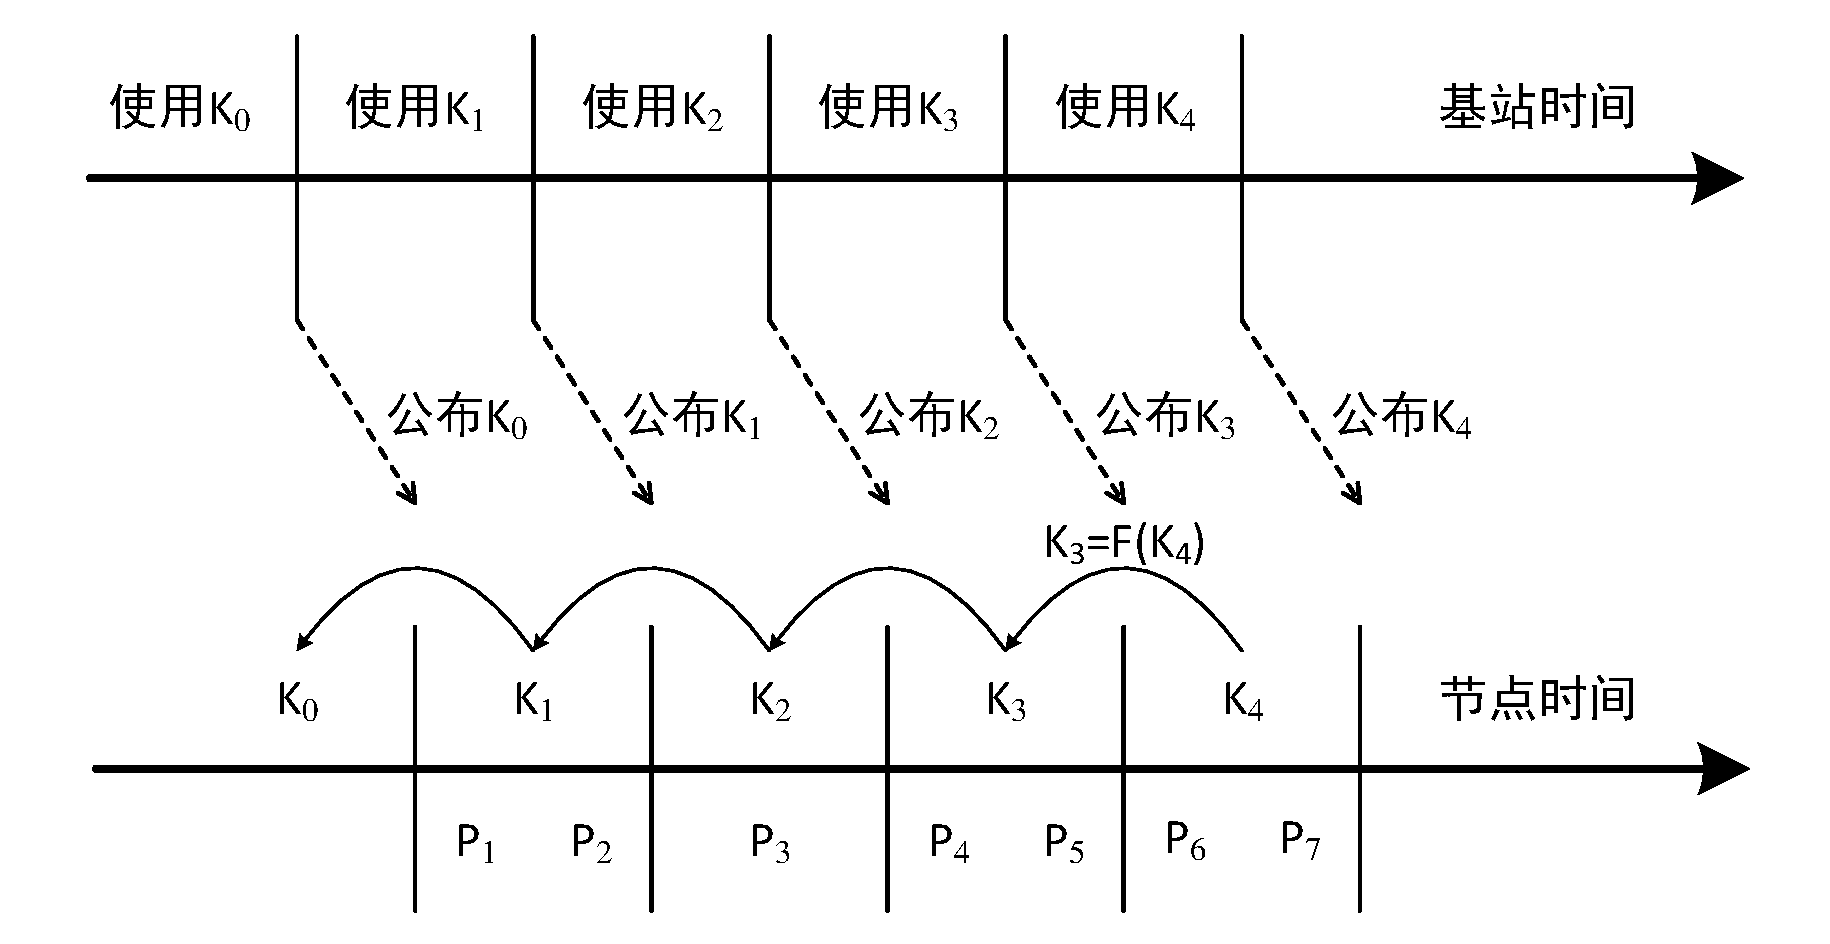
\includegraphics[width=5in]{TESLA}
  \caption{$\mu TESLA$认证机制}
  \label{fig:TESLA}
\end{figure}
如图~\ref{fig:TESLA}所示,是$\mu TESLA$方案的认证过程,$\mu TESLA$是基于对称密钥的,对报文计算消息认证码的认证密钥和节点对报文进行认证的密钥是相同的。其认证过程包括密钥建立、广播报文、自举接收者和对报文认证等步骤。其中密钥分发是通过单向hash 函数F 来实现的,如$K_3=F(K_4)$。 然后广播一个密钥$K_i$加密后的报文,无线传感网中基站和节点采用不同的时隙,使广播加密报文和接收到相应的密钥不同步。通过延迟发布密钥$K_i$,使得认证过程具有非对称性,提高认证的安全性能。通过比较报文的接收时间和认证密钥发布的时隙,能对报文的安全性进行检查。但该方案仍有其缺点:密钥的发布延后于报文的到达,因此节点接收到的报文必须缓存在节点中,浪费节点宝贵的存储空间,并且有可能被攻击者发动泛洪攻击,大量的伪造报文填满传感器节点的缓存空间,导致无线传感网传输功能失效,攻击者也容易发动虫洞攻击,威胁传感网的安全。

Liu等人基于$\mu TESLA$方案,提出了多级$\mu TESLA$方案\upcite{c1:MultiTesla},采用多级密钥链解决$\mu TESLA$方案中密钥链占用存储空间过大,容易导致泛洪攻击的问题。该方案使用预装初始化参数的方案,代替$\mu TESLA$方案中通过单播进行初始化的过程。如图~\ref{fig:MultiTESLA},是多级$\mu TESLA$方案的认证过程。在该方案中,Liu使用了2级时间,在1级时间中,将时间划分为$n_0$个间隔,每个时间间隔对应该级的单向hash链中的密钥$K_i,1\leq i \leq n_0$,其中密钥还是同$\mu TESLA$ 方案,使用单向hash链生成。一个1级时间间隔又被划分为$n_1$个2级时间间隔,每个2级时间间隔的密钥使用
$K_i,1\leq i \leq n_0$作为密钥种子生成。每个2级时间间隔内发送的报文用对应的密钥进行认证,其中的密钥链头$K_i,0$ 在前一个1级时间发布。
\begin{figure}[htbp]
  \centering
  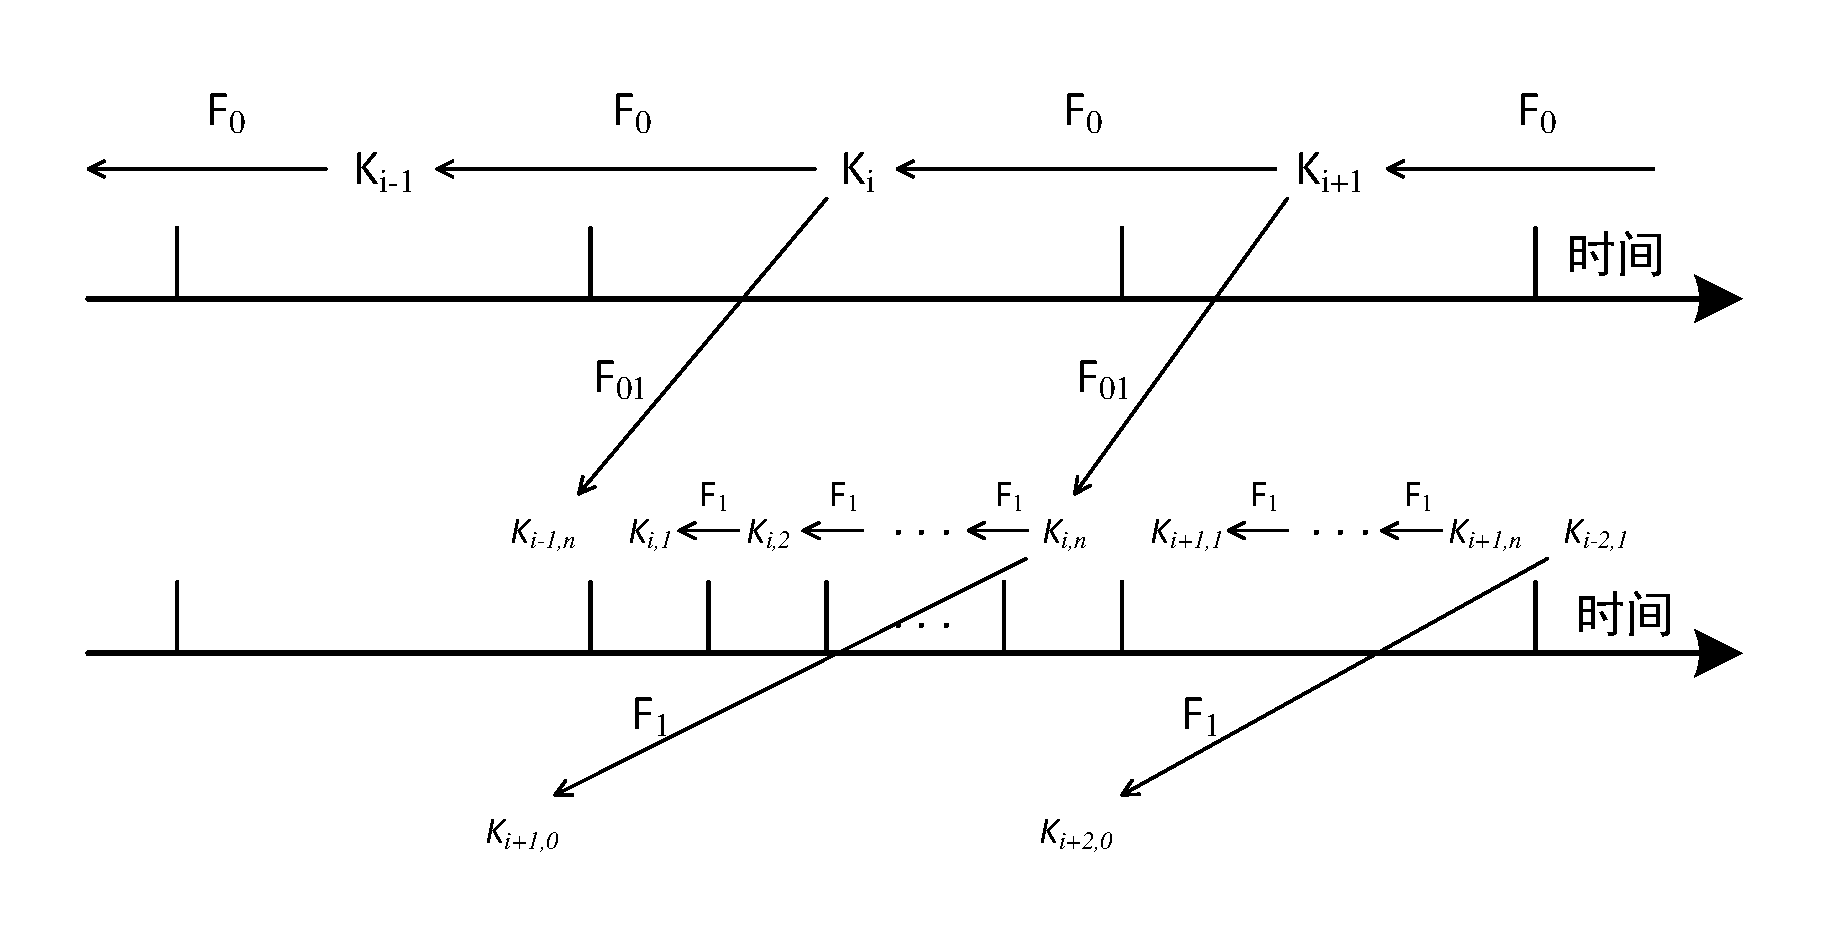
\includegraphics[width=5in]{multiTESLA}
  \caption{多级$\mu TESLA$认证机制}
  \label{fig:MultiTESLA}
\end{figure}

在裴庆祺等人的$\mu TESLA$改进方案中\upcite{c1:MMtesla},引入了$(t,n)$的门限秘密共享,每个认证密钥被分隔为$n$个密钥片,分配到各个基站。在无线传感网中执行原有的$\mu TESLA$方案,将密钥片进行广播,当一个节点接收到超过$t$个密钥片之后,就通过秘密共享的算法,对认证密钥进行恢复,重构出认证密钥。该方案提高了$\mu TESLA$方案的认证率,并且有高可靠性和高容忍性的特点,缺点是通信开销明显增加。

Anas等人提出了一种基于信任模型的认证方案\upcite{c1:anas},使用一个轻量级的基于椭圆曲线的简单认证密钥协议。通过通信实体之间建立信任级别,使非对称密钥认证系统能在资源有限的无线传感器节点上运行。

Dong等人利用消息预认证提出了一个基于密钥链的过滤方案\upcite{c1:verifyfilter},能对无线传感网中的广播进行过滤,有效减少虚假广播对传感网数据传输的影响,该方案的缺点是无法有效防御攻击者的联合节点攻击。




\subsection{无线传感网身份认证概述}

攻击者可以通过对网络发送大量的虚假数据报文,大量消耗节点的计算和存储能力,消耗节点的能量,导致传感网的失效。因此对传感网中的节点进行身份认证尤为重要。
文献\cite{c2:chan2003random}中,利用随机配对密钥分配方案,一个密钥仅会分配给一对节点,来实现一种非常简单的身份认证,即两个节点通过使用预分配的密钥对消息的加密和解密判断是否是经过认证的节点。但是该方案无法实现真正的身份认证,因为被捕获的节点可以伪装成正常节点进行欺骗,对无线传感网进行攻击。

现有的身份认证方案主要有非对称密钥认证和秘密共享认证。
由于无线传感器节点的限制,现阶段非对称密钥认证的实现一般是消耗能量较多的计算由基站完成,消耗能量较少的计算由节点完成。秘密共享的认证则是基于多个节点共同对一个节点进行认证。

虽然现阶段由于传感器节点的限制,非对称密钥没有被广泛应用于无线传感网的认证,但是许多研究也对此进行了探索。
在非对称密钥机制中,椭圆曲线密码(Elliptic Curve Cryptography,ECC)是一种轻量级的方案,研究结果表明,160位的ECC 能获得相当于1024位RSA密码的安全性能。而且使用非对称密钥不需要$\mu TESLA$方案中的延迟发布密钥,还能提高认证系统的安全性。

Watro等人提出了一个基于RSA算法的认证机制TinyPK\upcite{c1:Watro},该方案使用请求-应答机制。
该方案使用了双重校验,来保证认证机制的安全性。
当一个节点需要同另一个节点进行认证时,向该节点发送一个请求信息,其中包括两部分。第一部分是使用认证中心的私钥进行签名的请求节点的公钥,第二部分是使用请求节点私钥签名的时间戳和消息认证码。应答节点接收到该请求消息以后,使用认证中心的公钥对第一部分进行解密,获取请求节点的公钥。使用请求节点的公钥解密第二部分,获得时间戳和消息认证码,通过时间戳和消息认证码的校验,来判断请求节点的合法性。如果通过,则建立两个节点之间的安全通信。

在Bauer等人的方案\upcite{c1:Bauer}中,使用了秘密共享的思想进行身份认证。当一个节点请求对另一个节点的认证时,应答节点发送消息给认证中心,宣告自己被请求做认证处理,处理中心将请求节点的私钥进行划分,将秘密片广播给应答节点的邻居节点,所有节点发回给认证中心一个判定消息,如果通过认证的消息超过阈值,则请求节点通过认证,应答节点此时与认证中心进行交互,更新自己的私钥。

现有的身份认证方案还有Benenson提出的基于ECC的方案\upcite{c1:Benenson},Cao等基于vBNN-IBS提出的多用户广播认证方案\upcite{c1:Cao}。



\section{无线传感网密钥分配方案概述}

\subsection{无线传感网密钥分配概述}
无线传感网的密钥分配是其安全技术研究的一个重要内容,包括密钥预分发、共享密钥发现等研究方向。

无线传感网中的密钥分配与传统无线网络有较大区别,在传统的无线网络中,密钥分配方案的研究已经取得了许多成果,但是由于无法适应无线传感网的特点,这些成果无法应用于无线传感网中。因为WSN节点资源的限制,传统无线网络中节点计算开销和通信开销较大的密钥分配方案无法适用。在设计无线传感网的密钥分配方案时,不仅要保证方案的安全性能,也要权衡计算开销和通信开销。

进行认证的基础是密钥分配,设计一个面向无线传感网需求的密钥分配方案,才能保证认证机制的性能。
\subsection{无线传感网密钥分配方案分类}
近些年来,WSN的密钥分配有了许多新的研究成果,根据所适用的密钥是否是对称密钥,可以将方案分为对称密钥方案和非对称密钥方案。随着传感器技术的发展,非对称密钥技术可能成为将来无线传感器密钥分配的主流,但是由于目前无线传感器节点的计算能力和存储空间的限制,现有的无线传感网密钥分配以对称密钥方案为主。基于对称密钥,有很多的密钥分配机制的研究成果,表~\ref{tb:wsnkey}列出了目前无线传感网主要的密钥分配方案:

\begin{table}[htbp]
  \centering
  \caption{无线传感网主要的密钥分配方案}
  \label{tb:wsnkey}
  \begin{minipage}[t]{0.8\textwidth}
    \begin{tabularx}{\linewidth}{|c|X|X|}
      \hline
%      \multirow{1}*{网络层次}
%        & 常见的攻击 & 防范措施\\
      \multirow{1}*{数学结构}  & \multicolumn{1}{c|}{密钥分配方案} & \multicolumn{1}{c|}{密钥分配方法} \\
      \hline
      \multirow{3}*{密钥池}
        & E-G方案 & 随机预分发 \\\cline{2-2}
        & q-composite方案 & \\\cline{2-3}
        & PIKE方案 & 基于网格预分发\\
      \hline
      \multirow{4}*{二元对称多项式}
        & Blundo方案 & 确定预分发\\\cline{2-3}
        & Liu-Ning方案 & 基于随机子集预分发 \\\cline{2-3}
        & GBKP方案 & 基于网格预分发 \\\cline{2-3}
        & CPKS方案 & 基于位置预分发 \\
      \hline
      \multirow{2}*{MDS 码生成矩阵}
        & Blom方案 & 确定预分发 \\\cline{2-3}
        & Du-Deng方案 & 基于随机子集预分发 \\
      \hline
      \multirow{2}*{区组}
        & Camtepe方案 & 组合设计 \\\cline{2-3}
        & Camtepe混合组合设计方案 & 组合设计及随机预分发 \\
      \hline
    \end{tabularx}\\[2pt]
  \end{minipage}
\end{table}



\subsection{无线传感网典型密钥分配方案概述}
根据密钥分配方法的不同,我们对不同类别的无线传感网密钥分配方案进行概述:
\subsubsection{基于随机预分发的密钥分配}
Eschenauer和Gligor基于随机图理论,提出了无线传感网中随机密钥预分配的方案\upcite{c2:Eschenauer2002}(简称E-G方案),该方案包括3个阶段。在密钥预分发阶段,密钥分发中心生成一个足够大的密钥池$P$,然后对于每个传感器节点,从中随机选择$m$个不同的密钥,形成一个密钥环,并将密钥保存到传感器节点的存储空间中。在密钥发现阶段,每个节点通过相邻节点发现机制寻找物理上相邻的节点,由于所有节点的密钥是从密钥池中随机取出的,相邻节点可能存在相同的密钥,如果相邻节点存在共享密钥,则作为两者之间的会话密钥。当相邻节点之间不存在共享密钥,则开始路径密钥建立阶段。通过在密钥发现阶段建立的节点连通图$G(V,E)$(V为传感器节点的顶点集合,E为有共享密钥的传感器节点之间构成的边集),在图中查找一条通往没有共享密钥的相邻节点的路径,建立相邻节点之间的路径密钥。

在E-G方案中,两个相邻节点之间有共享密钥的概率$p$同节点存储密钥数$m$之间的关系可以表示为:$p=1-\frac{((P-m)!)^2}{(P-2m)!P!}$。E-G 方案使得每个节点只需要存储较小数量的密钥,就可以有较高概率使得无线传感器网络完成密钥建立过程,符合无线传感网的特点要求。但是E-G 方案作为最早提出的无线传感网密钥预分发方案,也有自身的缺点,当妥协节点增多时,无法保证无线传感网的通信安全,因为节点不具备防篡改的机制。而且当一个节点被捕获时,节点上存储的密钥材料全部都暴露给了攻击者,而且这些密钥可能是其他节点间的会话密钥,也就是使攻击者能攻击其他节点之间的通信。

在E-G方案的基础上,有许多方案对随机密钥预分配进行了改进,提升随机密钥预分配机制的性能。
Chan等人在E-G方案的基础上提出了q-composite 随机密钥预分配方案\upcite{c2:chan2003random},每个节点从密钥池$P$中获取$m$个不同的密钥。方案的密钥个数阈值为$q$,当两个节点之间的共享密钥个数$q^{'}$满足$q^{'}> q$,则两个节点之间使用hash函数$K=hash(K_1\| K_2\| \cdots \| K_{q^{'}})$生成会话密钥,在q-composite方案中,hash函数使用了SHA-1\cite{c2:sha1}。q-composite保证了相邻节点之间的安全链路,密钥个数阈值增大时,链路的安全性能也增大。在无线传感网被捕获节点较少时,该方案节点间链路的安全性能比E-G方案更好,但是当被捕获节点增多时,该方案的安全性能明显下降。


在Blom的对称密钥生成方案\upcite{c2:Blom84} 基础上,Du等人将其与随机密钥预分发结合,提出了无线传感网多密钥空间密钥预分发方案\upcite{c2:du2005pairwise}。先使用Blom方案生成$\omega$个密钥空间,每个节点从中选择$\tau$个密钥空间保证在存储空间中$(2 \leq \tau \leq \omega)$,如果两个节点上存储了一个相同的密钥空间,则他们之间计算生成一个共享密钥。与E-G 方案和q-composite方案相比,Du-Deng方案通过计算适合的参数$\omega$和$\tau$,能明显提高抵抗链路攻击的性能,但是同时也增加了节点的计算开销。

Blundo利用二元对称多项式的性质,提出了节点对密钥建立方案\upcite{c2:Blundo1998}。密钥服务器随机生成一个有限域上的$k$ 阶二元对称多项式$f(x,y)=\sum _{i,j=0}^k a_{i,j} x^i y^j$,对于对称多项式,有$f(x,y)=f(y,x)$。对于任意节点$i$,服务器计算$f(i,y)$,然后将$k+1$个系数存入节点存储空间。当节点$i$和节点$j$需要建立对密钥时,计算$f(i,y)$ 在$y=j$ 时的值,计算$f(j,y)$在$y=i$时的值,因为$f(i,j)=f(j,i)$,所以$f(i,j)$就可以作为节点$i$和节点$j$之间的对密钥。

在Blundo方案的基础上,Liu-Ning提出了基于对称二元多项式池的随机密钥预分配方案\upcite{c2:liu2005establishing}。
密钥服务器在有限域$F_q$上随机生成一个二元对称多项式的集合$\phi=\{f_i(x,y),i=1,\cdots,t\}$,对于节点$i$,将子集$\phi_i\subseteq \phi$装入存储空间。当两个节点发现有相同的二元多项式,则直接使用Blundo的节点对密钥建立方案建立会话密钥。当被捕获的节点较少时,Liu-Ning方案有较好的安全性能,但是在攻击者捕获了较多节点,也就是获得较多二元多项式的时候,链路的安全性能相较E-G方案和q-composite方案更低。

利用节点的位置信息,Liu提出了最近对密钥方案(CPKS)\upcite{c2:LiuN03},节点实际分布位置在其期望分布位置周围服从均匀分布。每个节点与自己期望分布位置最近的$t$节点之间建立对密钥,例如,对节点$u$的相邻节点$v$,密钥服务器生成对密钥$K_{u,v}$,并将$u,K_{u,v}$和$v,K_{u,v}$分别存入节点$u$和节点$v$。通过两个节点之间的ID信息可以判断两个节点之间是否存在对密钥。在节点位置信息已知时,该方案相比前述方案有更好的性能,缺点是网络扩展性较差,加入新节点,需要大量节点能量消耗。

Du提出的基于部署知识的方案\upcite{c2:Du06} 中,将密钥池$S$划分为$t\times n$的子密钥池$S_{i,j}(1\leq i\leq t,1\leq j\leq n)$,子密钥空间$S_{i,j}$对应着部署组$G_{i,j}$。根据部署位置的信息,不同的子密钥池之间发现共享密钥。该方案提高了无线传感网中节点链路连通的概率,但是子密钥池的划分对安全性能的影响较大。


\subsubsection{基于网格预分发的密钥分配}
为了解决随机密钥预分配方案中链路密钥的不确定性,Liu提出了基于网格的密钥预分配方案(GBKP)\upcite{c2:LiuND08}。
对一个$m\times n$的传感网,如图~\ref{fig:GBKP}所示,$G_i$为部署分组。对$G_i$中的节点分配ID集合$\{(i-1)m+j|j=1,\cdots,m\}$,对$G_i^{'}$中的节点分配ID集合$\{i+(j-1)m|i=1,\cdots,n\}$。服务器生成$m+n$个对称二元多项式分配给每行每列,使得同一行或同一列的节点能直接生成对密钥,不同行或列的节点,通过中间节点生成链路密钥。
类似的基于网格预分发的密钥分配方案还有Chan 提出的PIKE方案\upcite{c2:ChanP05}。
\begin{figure}[htbp]
  \centering
  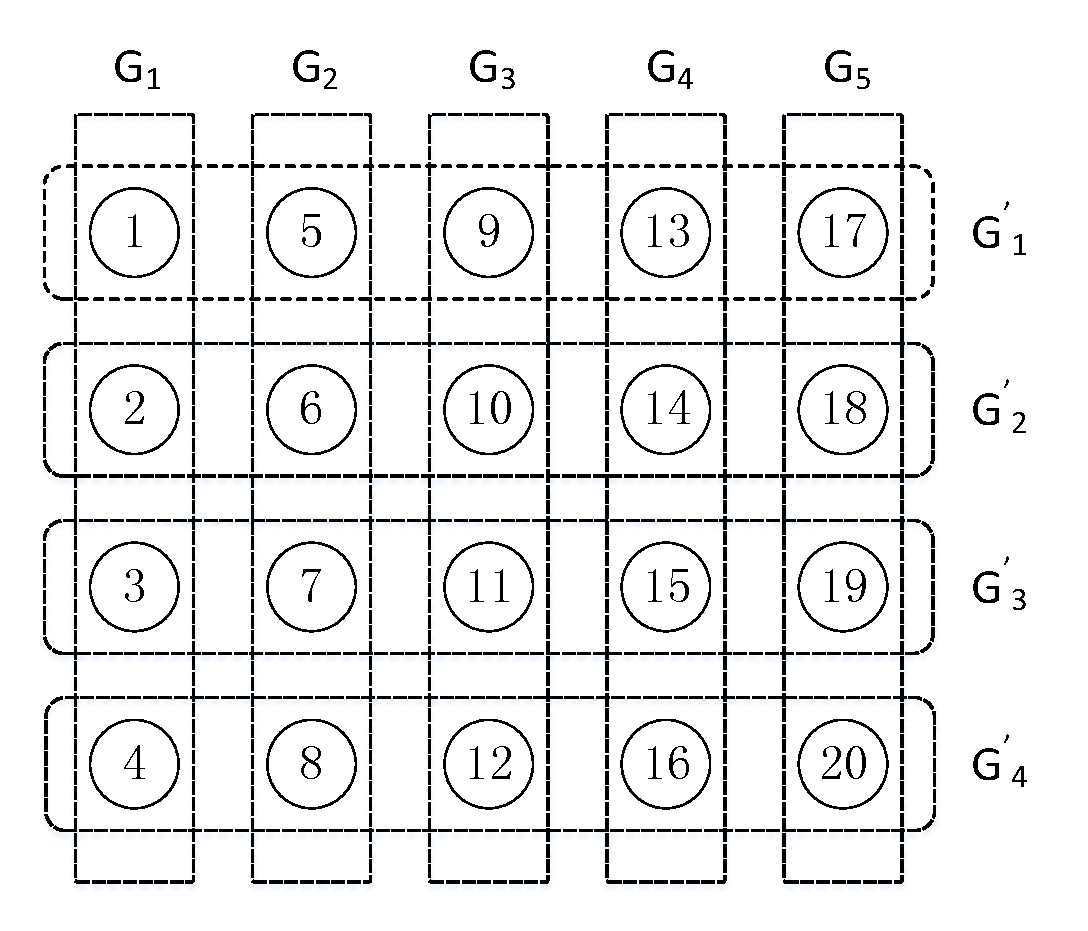
\includegraphics[width=4in]{GBKP}
  \caption{基于网格的密钥预分配方案}
  \label{fig:GBKP}
\end{figure}

\subsubsection{基于组合设计的密钥分配}
Camtepe把组合设计的理论应用于无线传感网的密钥分配\upcite{c2:CamtepeY07},使用组合设计理论来划分密钥池和密钥环。
对一个规模为$N$的无线传感网,生成一个对称BIBD,$(n^2+n+1,n+1,1)$,其中$n$为满足$n^2+n+1\geq N$的最小素数,密钥池的大小为$n^2+n+1$,密钥环的长度为$n+1$。这个方案保证了无线传感网中的任意一对节点有共享密钥,或通过中间节点生成的链路密钥。
为了解决该方案在网络规模方面的限制,Camtepe 还提出了组合设计与广义四边形想结合的方案。





%%% Local Variables:
%%% mode: latex
%%% TeX-master: "../main"
%%% End:

\begin{ack}
  衷心感谢导师 xxx 教授和 xxx 副教授对本人的精心指导。他们的言传身教将使我终生受益。

  感谢 \nudtpaper{},它的存在让我的论文写作轻松自在了许多,让我的论文格式规整漂亮了许多。

\end{ack}


%</thesis>
%    \end{macrocode}
%
% 在\LaTeX{}下管理参考文献将极其方便,建议使用Jabref生成条目,
% 用\verb|\cite|(其中\verb|upcite|是上标索引)索引即可。
% \verb|refs.bib|是你的参考文献名。
%    \begin{macrocode}
%<*thesis>
\cleardoublepage
\phantomsection
\addcontentsline{toc}{chapter}{参考文献}
\bibliographystyle{bstutf8}
\bibliography{ref/refs}

\begin{resume}

  \section*{发表的学术论文} % 发表的和录用的合在一起

  \begin{enumerate}[{[}1{]}]
  \addtolength{\itemsep}{-.36\baselineskip}%缩小条目之间的间距,下面类似
  \item Zongxiao Lan,Geming Xia,Aolong Zhou. Communication cost optimized session key transmission scheme for WSN based on non-perfect secret sharing. ICITMI, 2014.
  \end{enumerate}

\end{resume}

%</thesis>
%    \end{macrocode}
%
%<thesis>% 最后,需要的话还要生成附录,全文随之结束。
%    \begin{macrocode}
%<*thesis>
\appendix
\backmatter
% TeX
\chapter{模板提供的希腊字母命令列表}

大写希腊字母:
\begin{table}[htbp]
\centering
\begin{tabular}{llll}
\toprule
$\Gamma$~\verb|\Gamma| & $\Lambda$~\verb|\Lambda| & $\Sigma$~\verb|\Sigma| & $\Psi$~\verb|\Psi| \\
$\Delta$~\verb|\Delta| & $\Xi$~\verb|\Xi| & $\Upsilon$~\verb|\Upsilon| & $\Omega$~\verb|\Omega| \\
$\Theta$~\verb|\Theta| & $\Pi$~\verb|\Pi| & $\Phi$~\verb|\Phi| & \\
\midrule
$\varGamma$~\verb|\varGamma| & $\varLambda$~\verb|\varLambda| & $\varSigma$~\verb|\varSigma| & $\varPsi$~\verb|\varPsi| \\
$\varDelta$~\verb|\varDelta| & $\varXi$~\verb|\varXi| & $\varUpsilon$~\verb|\varUpsilon| & $\varOmega$~\verb|\varOmega| \\
$\varTheta$~\verb|\varTheta| & $\varPi$~\verb|\varPi| & $\varPhi$~\verb|\varPhi| & \\
\bottomrule
\end{tabular}
\end{table}

小写希腊字母:
\begin{table}[htbp]
\centering
\begin{tabular}{llll}
\toprule
$\alpha$~\verb|\alpha| & $\theta$~\verb|\theta| & $o$~\verb|o| & $\tau$~\verb|\tau| \\ 
$\beta$~\verb|\beta| & $\vartheta$~\verb|\vartheta| & $\pi$~\verb|\pi| & $\upsilon$~\verb|\upsilon| \\ 
$\gamma$~\verb|\gamma| & $\iota$~\verb|\iota| & $\varpi$~\verb|\varpi| & $\phi$~\verb|\phi| \\ 
$\delta$~\verb|\delta| & $\kappa$~\verb|\kappa| & $\rho$~\verb|\rho| & $\varphi$~\verb|\varphi| \\ 
$\epsilon$~\verb|\epsilon| & $\lambda$~\verb|\lambda| & $\varrho$~\verb|\varrho| & $\chi$~\verb|\chi| \\ 
$\varepsilon$~\verb|\varepsilon| & $\mu$~\verb|\mu| & $\sigma$~\verb|\sigma| & $\psi$~\verb|\psi| \\ 
$\zeta$~\verb|\zeta| & $\nu$~\verb|\nu| & $\varsigma$~\verb|\varsigma| & $\omega$~\verb|\omega| \\ 
$\eta$~\verb|\eta| & $\xi$~\verb|\xi| & $\varkappa$~\verb|\varkappa| & $\digamma$~\verb|\digamma| \\ 
\midrule
$\upalpha$~\verb|\upalpha| & $\uptheta$~\verb|\uptheta| & $\mathrm{o}$~\verb|\mathrm{o}| & $\uptau$~\verb|\uptau| \\ 
$\upbeta$~\verb|\upbeta| & $\upvartheta$~\verb|\upvartheta| & $\uppi$~\verb|\uppi| & $\upupsilon$~\verb|\upupsilon| \\ 
$\upgamma$~\verb|\upgamma| & $\upiota$~\verb|\upiota| & $\upvarpi$~\verb|\upvarpi| & $\upphi$~\verb|\upphi| \\ 
$\updelta$~\verb|\updelta| & $\upkappa$~\verb|\upkappa| & $\uprho$~\verb|\uprho| & $\upvarphi$~\verb|\upvarphi| \\ 
$\upepsilon$~\verb|\upepsilon| & $\uplambda$~\verb|\uplambda| & $\upvarrho$~\verb|\upvarrho| & $\upchi$~\verb|\upchi| \\ 
$\upvarepsilon$~\verb|\upvarepsilon| & $\upmu$~\verb|\upmu| & $\upsigma$~\verb|\upsigma| & $\uppsi$~\verb|\uppsi| \\ 
$\upzeta$~\verb|\upzeta| & $\upnu$~\verb|\upnu| & $\upvarsigma$~\verb|\upvarsigma| & $\upomega$~\verb|\upomega| \\ 
$\upeta$~\verb|\upeta| & $\upxi$~\verb|\upxi| & & \\ 
\bottomrule
\end{tabular}
\end{table}

希腊字母属于数学符号类别,请用\verb|\bm|命令加粗,其余向量、矩阵可用\verb|\mathbf|。


\end{document}
%</thesis>
%    \end{macrocode}
%
% 当然还有一些收尾工作,校验审阅自不必说。接下来你需要:修改论文中英文日期,
% 生成盲评,生成明(盲)评A3封面。
%
% {\color{blue}Happy \TeX{}ing! 欢迎提各式各样的意见!}
%
% \newpage\relax%
%
% \StopEventually{\PrintChanges}
% \clearpage
%
% \section{实现细节}
% 我们首先介绍文档模板的基本信息以及宏包和配置,
% 然后依照国防科学技术大学论文模板的书写规范一节一节的介绍实现步骤。
%
% \changes{v1.2}{2009/09/28}{添加了A3封面制作}
%
% \subsection{基本信息}
%    \begin{macrocode}
%<cls>\NeedsTeXFormat{LaTeX2e}[1999/12/01]
%<cls>\ProvidesClass{nudtpaper}
%<cfg>\ProvidesFile{nudtpaper.cfg}
%<cls|cfg>[2011/07/17 v2.2 NUDT paper template]
%    \end{macrocode}
%
% \subsection{宏包配置}
%
%<*cls>
%
%\changes{v0.99}{2009/08/17}{add package options}
% 当前的宏包选项在之前已经介绍了,下面是实现步骤,就是几个\verb|if|。
%\changes{v1.6}{2009/12/01}{添加单独的单双面控制}
%\changes{v2.0}{2010/11/09}{添加盲评控制}
%
%    \begin{macrocode}
\newif\ifismaster\ismastertrue
\newif\ifisttf\isttffalse
\newif\ifisfz\isfzfalse
\newif\ifisotf\isotffalse
\DeclareOption{master}{\ismastertrue}
\DeclareOption{doctor}{\ismasterfalse}
\newif\ifisanon\isanonfalse
\DeclareOption{anon}{\isanontrue}
\newif\ifistwoside\istwosidefalse
\DeclareOption{twoside}{\istwosidetrue}
\DeclareOption{ttf}{\isttftrue}
\DeclareOption{fz}{\isfztrue}
\DeclareOption{otf}{\isotftrue}
\newif\ifisvista\isvistafalse
\DeclareOption{vista}{\isvistatrue}
\DeclareOption*{\PackageWarning{nudtpaper}{Unknown Option '\CurrentOption'}}
\ProcessOptions\relax
%    \end{macrocode}
%
% 首先调用在文档类书写中需要的过程控制语句,在计算一些\verb|length|时要用到
%    \begin{macrocode}
\RequirePackage{ifthen,calc}
%    \end{macrocode}
%
% 接着我们导入文本类,该模板基于标准的书籍模板book,其默认格式为单面打印。
% 博士论文如需双面打印,必须指定\verb|twoside|选项。双开的含义是章节总是
% 起在右手边,左手空白页为完全的空白页,不包含页眉页脚。
%
% \changes{v1.6}{2009/12/01}{修改开关选项}
%
%    \begin{macrocode}
\ifistwoside
  \LoadClass[a4paper,12pt,openright,twoside]{book}
\else
  \LoadClass[a4paper,12pt,openany]{book}
\fi
%    \end{macrocode}
%
% 我们直接用\textsf{geometry}宏包进行页面边距的设定,调用titlesec设定标题以及页眉页脚,
% 用\textsf{titletoc}设定目录格式。需要改动的可以参考这三个宏包的说明文档。
%
%    \begin{macrocode}
\RequirePackage[includeheadfoot]{geometry}
\RequirePackage[center,pagestyles]{titlesec}
\RequirePackage{titletoc}
%    \end{macrocode}
%
% 文档中另外重要的两个部分是表格和图片。
% 首先来看图片:\textsf{graphicx}宏包是必不可少的,
% 并排图形。\textsf{subfigure} 已经不再推荐,用新的 \textsf{subfig}。
% 加入 \verb|config| 选项
% 以便兼容 \textsf{subfigure} 的命令。浮动图形和表格标题样式。\textsf{caption2} 已经不
% 推荐使用,采用新的 \textsf{caption}。它会自动被 \textsf{subfig} 装载进来。所以可以在
% 后面使用 \textbf{captionsetup} 命令,宏包\textsf{float}的作用是可以用H命令,
% 将浮动对象强制放在这里(副作用是版面可能不好):
%
%    \begin{macrocode}
\RequirePackage{graphicx}
\RequirePackage[config]{subfig}
\RequirePackage{float}
%    \end{macrocode}
%
% 再来看表格:我们采用\textsf{longtable}来处理长的表格,还需要\textsf{array}包;
% 标准的论文需要表格为三线表,这里引用\textsf{booktabs}宏包来处理,
% 这样,我们就可以简单的使用\verb|\toprule|,\verb|\midrule|,\verb|bottomrulle|
% 这样的命令;
% 为了在表格中支持跨行,需要引入\textsf{multirow}包,\textsf{tabularx}的作用是为了使用
% 固定宽度的表格,\textsf{slashbox}可以让我们在表格中使用反斜线:
%    \begin{macrocode}
\RequirePackage{array}
\RequirePackage{longtable}
\RequirePackage{booktabs}
\RequirePackage{multirow}
\RequirePackage{tabularx}
\RequirePackage{slashbox}
%    \end{macrocode}
% 表格和图片的例子可以搜索C\TeX{}论坛或者看示例文件。
%
% 引入\textsf{paralist}来达到比较好看的列表环境
%    \begin{macrocode}
\RequirePackage[neverdecrease]{paralist}
%    \end{macrocode}
%
% 文档中还需要一定的色彩控制和字体控制
%    \begin{macrocode}
\RequirePackage{xcolor}
%    \end{macrocode}
%
% 为了排出漂亮的数学公式,\textsf{amsmath}包是必不可少的,
% 需要注意的是,新版本的论文模板仍旧使用\textsf{txfonts}宏包,
% 为了支持希腊正体字母,需要调用\verb|upgreek.sty|,使用方法是\verb|\up<greek>|。
% 注意到这个宏包前面加上了\verb|Symbolsmallscale|选项,这是为了配合
% \verb|txfonts|希腊字体的大小而设定的。如果用户不满意这个宏包的积分号
% 等符号,倾向与使用传统的\LaTeX{}风格的数学符号,那么可以使用
% \textsf{mathptmx}宏包,但要把\verb|upgreek|的选项改为\verb|Symbol|,要不然
% 正体希腊字母要显得小一点哦。
% 而大写斜体希腊字母(变量)可以通过\textsf{amsmath}的\verb|\var<Greek>|得到。
% 当然,对于希腊字母的加粗推荐使用\verb|bm|宏包,一般变量的加粗那就使用
% \verb|\mathbf|吧!
% \changes{v2.0}{2010/11/09}{去掉fontspec,传递no-math到xeCJK,加入bm宏包}
% \changes{v2.2}{2011/07/16}{去掉txfonts宏包,使用lm字体,添加svgreek.sty}
% \changes{v2.2}{2011/07/16}{修改,仍旧使用upgreek, mathptmx, bm组合}
% \changes{v2.2}{2011/09/25}{修改,使用upgreek, txfonts, bm组合}
% \changes{v2.2}{2012/11/28}{给用户提供额外的选项,还是mtpro比较漂亮}
% \changes{v2.3}{2013/12/27}{调整数学字体,加入mtpro使用说明,并且仿照IEEE模板,修改displaypenalty}
%    \begin{macrocode}
\RequirePackage{amsmath,amssymb}
\RequirePackage{txfonts}
\RequirePackage[Symbolsmallscale]{upgreek}
%\RequirePackage{amsmath}
%\RequirePackage[amsbb,eufrak,compatiblegreek,subscriptcorrection,nofontinfo]{mtpro2}
\interdisplaylinepenalty=2500
\RequirePackage{bm}
\RequirePackage[T1]{fontenc}
\RequirePackage[amsmath,thmmarks,hyperref]{ntheorem}
%    \end{macrocode}
% 需要注意的是,如果用户有\verb|mtpro2|包,还是强烈建议使用这个的,因为数学公式
% 在这个包下显得特别的美观。虽然下载和安装不属于这篇使用说明的范畴,但是,上面的注释部分
% 可以给大家如何使用的一个简单的例子。当你安装好\verb|mtpro2|之后,主要取消注释,并且将
% 上面的三个包注释掉即可。
%
% 本文档类直接采用\XeTeX{}引擎,方便了字体配置以及编译,
% 这里需要调用\textsf{XeCJK}宏包,no--math的作用是不改变先前数学宏包设定的数学字体。
% 同时采用\textsf{indentfirst}宏包管理文字的缩进:
% \changes{v1.8}{2010/10/15}{修改了默认的xeCJK的选项,为了兼容旧的xeCJK版本,normalindentfirst选项暂不使用,而是在后面添加indentfirst包}
% \changes{v2.0}{2010/11/10}{传递no-math给xeCJK里面的fontspec宏包}
% \changes{v2.2}{2011/07/03}{移除CJKtextspace, CJKmathspace, CJKnumber选项}
%
%    \begin{macrocode}
\RequirePackage[CJKnumber,CJKchecksingle,no-math]{xeCJK}
\RequirePackage{indentfirst}
%    \end{macrocode}
%
% 另外一个关键部分是文献索引,包括书签以及参考文献的索引,记得\textsf{hyperref}配合
% \XeTeX{}使用时暂不能开启Unicode选项,新的发行版已经移除\textsf{hypernat}包。另外还要注意,你最终的打印版肯定
% 不希望有花花绿绿的链接,对吧?那就把下面那行\verb|hyperref|注释掉就行了。
% \changes{v2.1}{2010/12/29}{移除hypernat包}
% \changes{v2.2}{2011/07/17}{移除hyperref的CJKbookmarks旋向}
% \changes{v2.3}{2013/12/27}{加入色彩版hyperref}
%    \begin{macrocode}
\RequirePackage[numbers,sort&compress,square]{natbib}
\RequirePackage[colorlinks=true,linkcolor=blue,citecolor=red,pdfborder=0 1 1]{hyperref}
%\RequirePackage[pdfborder=0 0 1]{hyperref}
%    \end{macrocode}
%</cls>
%
%\subsection{基础配置}
% 本章主要介绍模板中用到的基本的元素和定义,现在包括两部分: 字体,字号和字体命令
%
%\subsubsection{字体定义}
% 我们首先来处理\TeX{}中最令人棘手的字体问题,
% 在使用\textsf{XeCJK}包之后,配置和选择很容易,
% 预先设定好一些字体命令是为了后面方便的更改文本字体的需要。
% 首先我们开启\TeX{}连字符:
%    \begin{macrocode}
%<*cls>
\defaultfontfeatures{Mapping=tex-text}
%</cls>
%    \end{macrocode}
%
% 之后用\textsc{XeCJK}包提供的命令设定字体,用户可以选择使用TTF还是OTF字体,
% Adobe的OpenType字体在排版上更具备优势,文档显示锐利,推荐使用。
% 另外在这一个新版本中,我们推荐用户也可以使用方正的字体,只要使用\verb|FZ|选项即可。
% 中注释掉相关的字体就可以。方正字体的有点是标点符号的位置无需修正,且字体之间配合很好。
% \verb|setcharclass|的作用是纠正xunicode、xeCJK的一些设定:
%
% \changes{v0.99}{2009/08/17}{add options TTF and OTF}
% \changes{v0.993}{2009/08/25}{加入VISTA用户选项}
% \changes{v1.9}{2010/10/28}{定义一个cusong字体,使用的是中宋}
% \changes{v2.3}{2013/12/27}{用户可以考虑使用方正字体,加入FZ选项}
%
%    \begin{macrocode}
%<*cls>
\xeCJKsetcharclass{"0}{"2E7F}{0}
\xeCJKsetcharclass{"2E80}{"FFFF}{1}
\newcommand\installTTF{%
  \setmainfont{Times New Roman}
  \setsansfont{Arial}
  \setmonofont{Courier New}
  \ifisvista
    \setCJKmainfont[BoldFont={SimHei},ItalicFont={KaiTi}]{SimSun}
    \setCJKmonofont{KaiTi} % Pluto use LiSu Thu use Kaiti, orig is SimSun
    \setCJKfamilyfont{fs}{FangSong}
    \setCJKfamilyfont{kai}{KaiTi}
  \else
    \setCJKmainfont[BoldFont={SimHei},ItalicFont={KaiTi_GB2312}]{SimSun}
    \setCJKmonofont{KaiTi_GB2312} % Pluto use LiSu Thu use Kaiti, orig is SimSun
    \setCJKfamilyfont{fs}{FangSong_GB2312}
    \setCJKfamilyfont{kai}{KaiTi_GB2312}
  \fi
  \setCJKsansfont{SimHei}
  \setCJKfamilyfont{song}{SimSun}
  \setCJKfamilyfont{hei}{SimHei}
  \setCJKfamilyfont{li}{LiSu}
  \setCJKfamilyfont{you}{YouYuan}
  \setCJKfamilyfont{cusong}{STZhongsong}
}
\newcommand\installOTF{%
  \setmainfont{Times New Roman} % could be changed to "Times New Roman PS Std" !!
  \setsansfont{Arial}
  \setmonofont{Courier New}
  \setCJKmainfont[BoldFont={Adobe Heiti Std},ItalicFont={Adobe Kaiti Std}]{Adobe Song Std}
  \setCJKsansfont{Adobe Heiti Std}
  \setCJKmonofont{Adobe Kaiti Std}
  \setCJKfamilyfont{song}{Adobe Song Std}
  \setCJKfamilyfont{hei}{Adobe Heiti Std}
  \setCJKfamilyfont{fs}{Adobe Fangsong Std}
  \setCJKfamilyfont{kai}{Adobe Kaiti Std}
  \setCJKfamilyfont{li}{Adobe Kaiti Std}
  \setCJKfamilyfont{you}{Adobe Kaiti Std}
  \setCJKfamilyfont{cusong}{STZhongsong}
}
\newcommand\installFZ{%
  \setmainfont{Times New Roman} % could be changed to "Times New Roman PS Std" !!
  \setsansfont{Arial}
  \setmonofont{Courier New}
  \setCJKmainfont[BoldFont={FZHei-B01},ItalicFont={FZKai-Z03}]{FZShuSong_GB18030-Z01}
  \setCJKsansfont{FZHei-B01} % Hei
  \setCJKmonofont{FZKai-Z03} % Kai
  \setCJKfamilyfont{song}{FZShuSong_GB18030-Z01}
  \setCJKfamilyfont{hei}{FZHei-B01}
  \setCJKfamilyfont{fs}{FZKai-Z03} % Kai
  \setCJKfamilyfont{kai}{FZKai-Z03} % Kai
  \setCJKfamilyfont{li}{FZKai-Z03} % Kai
  \setCJKfamilyfont{you}{FZKai-Z03} % Kai
  \setCJKfamilyfont{cusong}{FZXiaoBiaoSong-B05} % 小标宋
}
\newcommand{\cusong}{\CJKfamily{cusong}} % 中宋作为加粗宋体
%</cls>
%    \end{macrocode}
%
% \changes{v1.6}{2009/12/01}{替换OTF英文字体为标准Windows自带字体}
% \changes{v2.3}{2013/12/27}{添加FZ字体选项}
% 之后我们根据你的设定决定安装什么字体:
%
%    \begin{macrocode}
%<*cls>
\ifisttf
  \installTTF
\else
  \ifisfz
    \installFZ
  \else
    \installOTF
  \fi
\fi
%</cls>
%    \end{macrocode}
%
% 选定好字体之后,就是设定字体别名,这样我们就可以在文档的其他部分直接使用较短的命令来
% 指定特定的字体了:
%
%    \begin{macrocode}
%<*cls>
\newcommand{\song}{\CJKfamily{song}}    % 宋体
\newcommand{\fs}{\CJKfamily{fs}}        % 仿宋体
\newcommand{\kai}{\CJKfamily{kai}}      % 楷体
\newcommand{\hei}{\CJKfamily{hei}}      % 黑体
\newcommand{\li}{\CJKfamily{li}}        % 隶书
\newcommand{\you}{\CJKfamily{you}}      % 幼圆
\def\songti{\song}
\def\fangsong{\fs}
\def\kaishu{\kai}
\def\heiti{\hei}
\def\lishu{\li}
\def\youyuan{\you}
%</cls>
%    \end{macrocode}
%
% \subsubsection{字号定义}
%下面就是定义字号大小,这一部分我们有两个参考,其一是:
%
% \begin{verbatim}
% 参考科学出版社编写的《著译编辑手册》(1994年)
% 七号      5.25pt       1.845mm
% 六号      7.875pt      2.768mm
% 小五      9pt          3.163mm
% 五号      10.5pt       3.69mm
% 小四      12pt         4.2175mm
% 四号      13.75pt      4.83mm
% 三号      15.75pt      5.53mm
% 二号      21pt         7.38mm
% 一号      27.5pt       9.48mm
% 小初      36pt         12.65mm
% 初号      42pt         14.76mm
%
% 这里的 pt 对应的是 1/72.27 inch,也就是 TeX 中的标准 pt
% \end{verbatim}
%
% 另外一个来自WORD中的设定:
% \begin{verbatim}
% 初号 = 42bp = 14.82mm = 42.1575pt
% 小初 = 36bp = 12.70mm = 36.135 pt
% 一号 = 26bp = 9.17mm = 26.0975pt
% 小一 = 24bp = 8.47mm = 24.09pt
% 二号 = 22bp = 7.76mm = 22.0825pt
% 小二 = 18bp = 6.35mm = 18.0675pt
% 三号 = 16bp = 5.64mm = 16.06pt
% 小三 = 15bp = 5.29mm = 15.05625pt
% 四号 = 14bp = 4.94mm = 14.0525pt
% 小四 = 12bp = 4.23mm = 12.045pt
% 五号 = 10.5bp = 3.70mm = 10.59375pt
% 小五 = 9bp = 3.18mm = 9.03375pt
% 六号 = 7.5bp = 2.56mm
% 小六 = 6.5bp = 2.29mm
% 七号 = 5.5bp = 1.94mm
% 八号 = 5bp = 1.76mm
%
% 1bp = 72.27/72 pt
% \end{verbatim}
%
% 我们采用习惯的字号设定方法(也就是WORD中的设定),首先编写字体设置命令:
%
%\begin{macro}{\choosefont}
% 我们可以使用 |\choosefont| 来选择字体, 字体设定这些大多是从清华的模板拷过来的。
%
%    \begin{macrocode}
%<*cls>
\newlength\thu@linespace
\newcommand{\thu@choosefont}[2]{%
    \setlength{\thu@linespace}{#2*\real{#1}}%
    \fontsize{#2}{\thu@linespace}\selectfont}
\def\thu@define@fontsize#1#2{%
    \expandafter\newcommand\csname #1\endcsname[1][\baselinestretch]{%
    \thu@choosefont{##1}{#2}}}
%</cls>
%    \end{macrocode}
%\end{macro}
%
%设定具体的字体大小:
%
%    \begin{macrocode}
%<*cls>
\thu@define@fontsize{chuhao}{42bp}
\thu@define@fontsize{xiaochu}{36bp}
\thu@define@fontsize{yihao}{26bp}
\thu@define@fontsize{xiaoyi}{24bp}
\thu@define@fontsize{erhao}{22bp}
\thu@define@fontsize{xiaoer}{18bp}
\thu@define@fontsize{sanhao}{16bp}
\thu@define@fontsize{xiaosan}{15bp}
\thu@define@fontsize{sihao}{14bp}
\thu@define@fontsize{banxiaosi}{13bp}
\thu@define@fontsize{xiaosi}{12bp}
\thu@define@fontsize{dawu}{11bp}
\thu@define@fontsize{wuhao}{10.5bp}
\thu@define@fontsize{xiaowu}{9bp}
\thu@define@fontsize{liuhao}{7.5bp}
\thu@define@fontsize{xiaoliu}{6.5bp}
\thu@define@fontsize{qihao}{5.5bp}
\thu@define@fontsize{bahao}{5bp}
%</cls>
%    \end{macrocode}
%
%\subsubsection{自定命令}
% 有一些常量,测试,自定义的命令等都放在这里,待到论文逐渐完善之后再做定夺,
% 当然用户自己的命令也可以在此添加,事实上如果natbib传递的是superscript,
% \verb|cite|命令默认就成了上标了。这里不加入这个选项,而是单独编写一个命令:
%
%    \begin{macrocode}
%<*cls>
\newcommand{\upcite}[1]{\textsuperscript{\cite{#1}}} % 上标形式引用
\newcommand{\china}{中华人民共和国}
\def\nudtpaper{\textsc{Nudt}\textsc{Paper}}
\newcommand{\pozhehao}{\kern0.3ex\rule[0.8ex]{2em}{0.1ex}\kern0.3ex}
%</cls>
%    \end{macrocode}
%
%\subsubsection{中文元素}
%
% 默认的页面元素的英文名,诸如Contents为目录,Abstract为摘要等,
% 我们首先将他们一一中文化:
% \changes{v0.992}{2009/08/19}{修改图表编号格式}
% \changes{v1.3}{2009/10/14}{修改图目录和表目录}
%
%    \begin{macrocode}
%<*cls>
\renewcommand\contentsname{目\hspace{1em}录}
\renewcommand\listfigurename{图\hspace{1em}目\hspace{1em}录}
\renewcommand\listtablename{表\hspace{1em}目\hspace{1em}录}
\newcommand\listequationname{公式索引}
\newcommand\equationname{公式}
\renewcommand\bibname{参考文献}
\renewcommand\indexname{索引}
\renewcommand\figurename{图}
\renewcommand\tablename{表}
\renewcommand\appendixname{附录}
\def\CJK@today{\CJKdigits{\the\year} 年 \CJKnumber{\the\month} 月}
\newcommand\zhtoday{\CJK@today}
\newcommand\entoday{\today{}}
%</cls>
%    \end{macrocode}
%
% 好,下面就开始按照论文模板要求进行排版!
%
%\subsection{编写要求}
% 学校规定,论文需采用白色纸双面打印。
% 学位论文用A4($210mm\times{}297mm$)标准大小的白纸,
% 在打字或印刷时,要求纸的四周留足空白边缘,以便装订、复制和读者批注。
% 每一面的上方(天头)和下方(地角)分别留边25mm,左侧(订口)
% 和右侧(切口)分别留边30mm,页眉与页脚分别为23mm。
%
% 实现起来很简单,只要调用\textsf{geometry}的版面控制命令即可,
% 方法为先把word模板转化为PDF,
% 用Adobe的裁剪功能查看页边距,进行微调,直到比对正确为止,设定如下:
%
% \changes{v0.991}{2009/08/18}{modify bottom skip}
% \changes{v1.1}{2009/09/26}{修改footskip容限以及bottom的值,为了容下longtab的''下一页''}
% \changes{v1.4}{2009/10/28}{减小页眉skip 1mm,用word叠印}
% \changes{v1.4}{2009/10/30}{增大页眉sep .5mm,用word叠印}
%
%    \begin{macrocode}
%<*cls>
\geometry{top=21mm,bottom=25.5mm,left=30mm,right=30mm}
\geometry{headheight=9mm,headsep=1mm,footskip=9mm}
%</cls>
%    \end{macrocode}
%
%\subsection{页眉页脚}
%
% 我们采用titlesec进行页面配置。
% 页面中的主要元素有Chapter,Section,Subsection等元素的外观,
% 位置,颜色字体等,页面元素还包括页眉页脚。这种方法配置简便,易管理。
% 国防科大的论文需要在页眉处画两根横线,我们通过下面的命令实现:
%
%\begin{macro}{\setheadrule}
% 这个命令属于更改\textsf{titlesec}中的一个画页眉的命令,稍加调整:
% \changes{v0.991}{2009/08/18}{modify headrull, s.t. all geometry match}
% \changes{v1.9}{2010/10/28}{去掉headsep,修改headrule,在sethead后添加raisebox}
%
%    \begin{macrocode}
%<*cls>
\renewcommand\setheadrule[1]{%
  \ifdim#1=\z@
    \let\makeheadrule\@empty
  \else
    \def\makeheadrule{%
    \makebox[0pt][l]{\rule[.2\baselineskip]{\linewidth}{1.5pt}}%
    \rule{\linewidth}{1.5pt}}%
  \fi}
%</cls>
%    \end{macrocode}
%\end{macro}
%
% 由于Chapter第一页默认是\verb|plain|页面格式,
% 章节的其余部分是在Matter中设定的页面格式,为了简单起见,
% 我们就直接更改\verb|plain|页面设置,
% 要求为5号宋体居中放置,画页眉页脚,页脚为1磅黑线
%
% \changes{v0.992}{2009/08/20}{renewpagestyle里面前导的空格可能导致clearpage生成新的一页,将空格去掉}
% \changes{v0.993}{2009/08/26}{修改标题,博士硕士对应不同的页眉}
%
%    \begin{macrocode}
%<*cls>
\renewpagestyle{plain}{
\sethead{}{\raisebox{.65\baselineskip}{\songti \wuhao \ifisanon{~}\else{国防科学技术大学研究生院\@optionpaperclass{}学位论文}\fi}}{}%
\setfoot{}{{\songti \wuhao 第~\thepage~页}}{}%
\headrule%
\footrule%
}
\setfootrule{1bp}
%</cls>
%    \end{macrocode}
%
%\subsection{编写格式}
%
% 当页面设置好之后,就是在论文的不同部分分别调用,一般来说论文类的书籍
% 分为三个matter,为前言区(前置部分),正文区(主体),后文区(附录),
% 在国防科大论文书写要求中,
% 需要将摘要单独进行页码编号,其编号为小写罗马字母,为此,
% 可以将摘要单独设定为一个matter,
% 名叫就叫做MidMatter,称作摘要区。每个Matter我们都一一介绍。
%
% 首先看前置部分,主要包括封面,目录,摘要等,实现为:
%
%    \begin{macrocode}
%<*cls>
\renewcommand\frontmatter{%
    \if@openright\cleardoublepage\else\clearpage\fi
    \@mainmatterfalse
    \pagenumbering{Roman}
    \pagestyle{plain}}
\newcommand\midmatter{%
    \if@openright\cleardoublepage\else\clearpage\fi
    \@mainmatterfalse
    \pagenumbering{roman}
    \pagestyle{plain}}
%</cls>
%    \end{macrocode}
%
% 之后为文章的正文区,采用阿拉伯数字编页码:
%
%    \begin{macrocode}
%<*cls>
\renewcommand\mainmatter{%
    \if@openright\cleardoublepage\else\clearpage\fi
    \@mainmattertrue
    \pagenumbering{arabic}
    \pagestyle{plain}}
%</cls>
%    \end{macrocode}
%
% 最后是附录部分,由于他的章节标题与正文中不一样(不是第几章,而是附录几),
% 我们需要单独设定:
%
%    \begin{macrocode}
%<*cls>
\renewcommand\backmatter{%
    \if@openright\cleardoublepage\else\clearpage\fi
    \titleformat{\chapter}{\filcenter \heiti \sanhao}{附录\,\thechapter\,}{1em}{}
    \titlecontents{chapter}[0pt]{\vspace{0.25\baselineskip} \heiti \xiaosi[1.25]}
      {附录\,\thecontentslabel\quad}{}
      {\hspace{.5em}\titlerule*{.}\contentspage}
    \@mainmattertrue
    \pagestyle{plain}}
%</cls>
%    \end{macrocode}
%
% 我们重新定义\verb|cleardoublepage|,使得生成完全的空白页,页面模式为\verb|empty|
%    \begin{macrocode}
%<*cls>
\renewcommand\cleardoublepage{\clearpage\if@openright \ifodd\c@page\else
  \newpage{}
  \thispagestyle{empty}
  \vspace*{\fill}
  \begin{center}
  \end{center}
  \vspace*{\fill}
  \clearpage\fi\fi%
}
%</cls>
%    \end{macrocode}
%
%\subsubsection{前置目录}
% 前置部分的封面在后面详细介绍。首先看目录,要求为:
% 目次页由论文的章、节、条、项、附录等的序号、名称和页码组成,
% 另页排在序之后。目次页标注学位论文的前三级目录。
% 标题统一用“目录”,黑体3字号字居中,段前、段后间距为1行;
% 各章(一级目录)名称用黑体小4号字,段前间距为0.5行,
% 段后间距为0行; 其它(二、三级目录)用宋体小4号字,
% 段前、段后间距为0行。:
%
% 在\LaTeX{}中,Chapter在目录中默认是没有点的,我们加上,另外我们一并将
% 目录中的section和subsection设定好,
% \changes{v0.991}{2009/08/18}{modify TOC baselineskip and font lineskip to 1.25}
%
%    \begin{macrocode}
%<*cls>
\titlecontents{chapter}[0pt]{\vspace{0.25\baselineskip} \heiti \xiaosi[1.25]}
    {第\CJKnumber{\thecontentslabel}章\quad}{}
    {\hspace{.5em}\titlerule*{.}\contentspage}
\titlecontents{section}[2em]{\songti \xiaosi[1.25]}
    {\thecontentslabel\quad}{}
    {\hspace{.5em}\titlerule*{.}\contentspage}
\titlecontents{subsection}[4em]{\songti \xiaosi[1.25]}
    {\thecontentslabel\quad}{}
    {\hspace{.5em}\titlerule*{.}\contentspage}
%</cls>
%    \end{macrocode}
%
% 然后是表目录和图目录,内容用宋体小4号字,在同学使用模板时,需要标题对齐,
% 我们一并在这里实现:
% \changes{v0.993}{2009/08/25}{添加makebox使得图表标题对齐}
%
%    \begin{macrocode}
%<*cls>
\titlecontents{figure}[0pt]{\songti \xiaosi[1.25]}
    {\makebox[3.5em][l]{图~\thecontentslabel\quad}}{}
    {\hspace{.5em}\titlerule*{.}\contentspage}
\titlecontents{table}[0pt]{\songti \xiaosi[1.25]}
    {\makebox[3.5em][l]{表~\thecontentslabel\quad}}{}
    {\hspace{.5em}\titlerule*{.}\contentspage}
%</cls>
%    \end{macrocode}
%
% 书籍模板中,在LOF或者LOT章节之间会默认插入额外的距离,我们通过修改下面这个命令移除,
% 这个方法不是一个完美的办法,\textbf{注意}:下面的代码不要去深究或者理解,
% 这只是把book.cls中的内容复制过来,然后去掉包含addvspace命令的两行。
% 我实在找不出更加好的办法,如果你有,可以联系我。
%
% \changes{v0.993}{2009/08/25}{移除LOF及LOT中章节之间额外的距离}
%
%    \begin{macrocode}
%<*cls>
\renewcommand\chapter{\if@openright\cleardoublepage\else\clearpage\fi
                    \thispagestyle{plain}%
                    \global\@topnum\z@
                    \@afterindentfalse
                    \secdef\nudt@chapter\@schapter}
\def\nudt@chapter[#1]#2{
  \ifnum \c@secnumdepth >\m@ne
    \if@openright\cleardoublepage\else\clearpage\fi
    \phantomsection
    \if@mainmatter
      \refstepcounter{chapter}%
      \addcontentsline{toc}{chapter}%
        {\protect\numberline{\thechapter}#1}%
    \else
      \addcontentsline{toc}{chapter}{#1}%
    \fi
  \else
    \addcontentsline{toc}{chapter}{#1}%
  \fi
  \chaptermark{#1}%
  \if@twocolumn
    \@topnewpage[\@makechapterhead{#2}]%
  \else
    \@makechapterhead{#2}%
    \@afterheading
  \fi
}
%</cls>
%    \end{macrocode}
%
%\subsubsection{前置摘要}
%
% 摘要的要求为题目黑体3字号字居中,段前、段后间距为1行,内容用宋体小4号字,
% 英文摘要内容用Time New Roman小4号字。
% 中文关键字以黑体小4号字另起一行,排在摘要的下方,英文关键字用Arial小4号字。
%
% \changes{v1.8}{2010/10/15}{ABSTRACT和英文关键字需要用Arial字体}
%    \begin{macrocode}
%<*cls>
\newcommand\cabstractname{摘\hspace{1em}要}
\newcommand\eabstractname{ABSTRACT}
\newcommand\ckeywordsname{关键词}
\newcommand\ckeywords[1]{{\hei\xiaosi \ckeywordsname: #1}}
\newcommand\ekeywordsname{Key Words}
\newcommand\ekeywords[1]{\textsf{\xiaosi \ekeywordsname: #1}}
\newenvironment{cabstract}{%
    \chapter{\cabstractname}
    \xiaosi
    \@afterheading}
    {\par\vspace{2em}\par}
\newenvironment{eabstract}{%
    \chapter{\textsf{\eabstractname}}
    \xiaosi
    \@afterheading}
    {\par\vspace{2em}\par}
%</cls>
%    \end{macrocode}
%
%\subsection{主体部分}
%
% \subsubsection{标题格式}
% 要求为:
% \begin{compactenum}
% \item	一级标题(章)用黑体3号字居中,1.25倍行距,段前、段后间距为1行,每一章从新的一页开始;
% \item	二级标题(节)用宋体4号粗体字居中,1.25倍行距,段前、段后间距为1行;
% \item	三级标题用黑体小4号字两端对齐,1.25倍行距,段前、段后间距为1行;
% \item	四级标题用宋体小4号粗体字两端对齐,1.25倍行距,段前间距为0.5行,段后间距为0行;
% \end{compactenum}
%
% \changes{v0.991}{2009/08/18}{按照要求设定标题}
% \changes{v0.992}{2009/08/19}{修改secnumdepth使得subsubsection可用}
% \changes{v1.1}{2009/09/26}{修改Title的spacing为弹性值}
% \changes{v1.2}{2009/10/06}{去掉弹性值,不去生成大量的空白}
% \changes{v1.4}{2009/10/28}{修改chapter段后行距为2ex,段前-1ex,保证上下对称}
% \changes{v1.4}{2009/10/29}{修改chapter段后行距为2.4ex,段前-1.2ex,保证上下对称}
%
% 当章节标题出现的新的一页时,会出现段前距过小的情况,按照milksea的说法是:
% 一般而言,当一个内容在一页开头时,前面的\verb|\vskip|不起作用;
% 类似地,一行开头\verb|\hskip|不起作用。这不是 BUG,如果需要总起效果的间距,
% 用\verb|\vspace*|,文档里面有这样的例子。参照titlesec的文档,需加上:
% \changes{v1.9}{2010/10/28}{增加sectionbreak,设定topskip为0pt}
%
%    \begin{macrocode}
%<*cls>
\newcommand{\sectionbreak}{%
\addpenalty{-300}%
\vspace*{0pt}%
}
\setlength{\topskip}{0pt}
%</cls>
%    \end{macrocode}
% \changes{v1.9}{2010/10/28}{在定义了粗宋字体之后,按照学位论文要求设定标题字体}
% \changes{v1.9}{2010/10/28}{使用了ttltips.pdf的设置chapter距顶端距离的办法}
% \changes{v2.3}{2013/12/27}{修改了footnotesize,当一页中有两个footnote时,间距调整正常}
% \changes{v2.3}{2013/12/27}{修改了titleformat和titlespacing的定制,更改英文字体,修正间距}
%
%    \begin{macrocode}
%<*cls>
\setcounter{secnumdepth}{3}
\setlength{\footnotesep}{2.2ex \@minus 2bp}
\titleformat{\chapter}{\filcenter\sf \heiti\sanhao[1.25]}{第\CJKnumber{\thechapter}章\,}{1em}{}
\titleformat{\section}{\filcenter\bfseries \cusong\sihao[1.25]}{\thesection}{1em}{}
\titleformat{\subsection}{\sf \heiti\xiaosi[1.25]}{\thesubsection}{1em}{}
\titleformat{\subsubsection}{\bfseries \cusong\xiaosi[1.25]}{\thesubsubsection}{1em}{}
\titlespacing{\chapter}{0pt}{2.4ex-\topskip-\heightof{A}}{2.4ex \@minus 2bp}
\titlespacing{\section}{0pt}{2ex-\heightof{a}}{2ex \@minus 2bp}
\titlespacing{\subsection}{2em}{2ex \@minus 2bp}{2ex \@minus 2bp}
\titlespacing{\subsubsection}{2em}{1ex \@minus 2bp}{0ex \@minus 2bp}
%</cls>
%    \end{macrocode}
%
%\subsubsection{正文字体}
% 首先确定正文中使用的字体,文档要求正文字体为小四,行距为固定值1.25倍,
% 中文字体为宋体,英文为{Times New Roman}
%
%\begin{macro}{\normalsize}
% 我们重新定义 |\normalsize| 来确定文档的正文字体,
% 同时修改正文中公式与文字间的距离:
% \changes{v1.9}{2010/10/28}{在normalsize后面每一行加上\%号来吃掉多余的空格}
% \changes{v2.2}{2011/07/16}{减小公式之间距离rubber space的上界}
% \changes{v2.2}{2011/09/25}{减小公式之间距离rubber space的下界}
% \changes{v2.3}{2013/12/27}{移除了abovedisplay的正向rubberspace}
%
%    \begin{macrocode}
%<*cls>
\renewcommand\normalsize{%
\@setfontsize\normalsize{12bp}{12.87bp}%
\renewcommand{\baselinestretch}{1.3}%
\setlength\abovedisplayskip{10bp \@minus 1bp}%
\setlength\abovedisplayshortskip{10bp \@minus 1bp}%
\setlength\belowdisplayskip{\abovedisplayskip}%
\setlength\belowdisplayshortskip{\abovedisplayshortskip}%
}
%</cls>
%    \end{macrocode}
%\end{macro}
%
% \changes{v0.991}{2009/08/18}{modify normalsize, which will cause headrule shift}
% \changes{v0.991}{2009/08/18}{add comment on displayskip}
% \changes{v1.0}{2009/09/22}{modify display skip}
%
%\subsubsection{正文段落}
% 接下来还有一个细节就是处理段落缩进,文档设定为首行缩进2个字符,
% 这一个命令需要在文档开始时自动执行:
%
% \changes{v1.3}{2009/10/03}{添加checkparameter这一选项,避免由于更新模板导致未定义的情况出现}
% \changes{v1.7}{2010/04/30}{应当在封面制作完后替换tabular}
%
%    \begin{macrocode}
%<*cls>
\newlength\CJK@twochars
\def\CJK@spaceChar{\Unicode{48}{7}}
\def\CJKindent{%
  \settowidth\CJK@twochars{中国}%
  \parindent\CJK@twochars}
\AtBeginDocument{%
  \CJKindent\relax
  \checkparameter\relax
}
%</cls>
%    \end{macrocode}
%
% 之后定义段落间距,段前间距以及段后间距都为0
% \changes{v0.993}{2009/08/27}{修改parskip}
% \changes{v2.2}{2011/09/25}{修改parskip,允许少量的调整,1bp}
% \changes{v2.2}{2011/10/14}{修改parskip,仅允许负的少量调整,2bp}
% \changes{v2.3}{2013/12/27}{移除parskip的正向rubberspace}
%
%    \begin{macrocode}
%<*cls>
\setlength{\parskip}{0bp \@minus 2bp}
%</cls>
%    \end{macrocode}
%
% 有时候我们需要手动设定字体间距,该命令在声明页使用过:
%\begin{macro}{\ziju}
%    \begin{macrocode}
%<*cls>
\newcommand*{\ziju}[1]{\renewcommand{\CJKglue}{\hskip #1}}
%</cls>
%    \end{macrocode}
%\end{macro}
%
% \changes{v1.4}{2009/10/26}{推荐用户使用紧凑的列表环境}
%
% 这一部分来自Thuthesis的代码,其出发点是不满意\LaTeX{}默认列表环境间距过大,用
% paralist包中的相关环境进行替代。请参考paralist宏包。
%
% \changes{v1.4}{2009/10/26}{修改参考文献的行距设定}
%
% 而同样有间距问题的是参考文献,两个条目之间过大的距离不是很美观,
% 最简单的办法是修改bibsep变量,如果还是不行,我们直接从thuthesis中拿来代码:
%
% \changes{v1.4}{2009/10/26}{修改参考文献的行距}
% \changes{v1.4}{2009/10/29}{修改参考文献左对齐}
% \changes{v2.2}{2011/10/14}{减小文献列表间距,将penalty改为4000}
%
%    \begin{macrocode}
%<*cls>
\renewenvironment{thebibliography}[1]{%
   \chapter*{\bibname}%
   \list{\@biblabel{\@arabic\c@enumiv}}%
        {\renewcommand{\makelabel}[1]{##1\hfill}
         \settowidth\labelwidth{1.1cm}
         \setlength{\labelsep}{0.4em}
         \setlength{\itemindent}{0pt}
         \setlength{\leftmargin}{\labelwidth+\labelsep}
         \addtolength{\itemsep}{-0.7em}
         \usecounter{enumiv}%
         \let\p@enumiv\@empty
         \renewcommand\theenumiv{\@arabic\c@enumiv}}%
    \sloppy\frenchspacing
    \clubpenalty4000%
    \widowpenalty4000%
    \interlinepenalty4000%
    \sfcode`\.\@m}
   {\def\@noitemerr
     {\@latex@warning{Empty `thebibliography' environment}}%
    \endlist\frenchspacing}
%</cls>
%    \end{macrocode}
%
%\subsection{浮动对象}
%
% 浮动对象针对的目标是图片表格,标题为五号字体,
% 图片标题在下,表格标题在上,具体实现为:
% \changes{v1.1}{2009/09/26}{修改float浮动弹性}
% \changes{v2.2}{2011/09/25}{去掉1.0fil改为4bp, 这样不至于生成过大的空白.}
% \changes{v2.3}{2013/12/27}{移除了floatsep所有rubberspace. 原先为正2负2.}
%
%    \begin{macrocode}
%<*cls>
\setlength{\floatsep}{12bp}
\setlength{\intextsep}{12bp}
\setlength{\textfloatsep}{12bp}
\setlength{\@fptop}{0bp}
\setlength{\@fpsep}{12bp}
\setlength{\@fpbot}{0bp}
%</cls>
%    \end{macrocode}
%
% 接下来设置每一页图形占据的比例,这个直接从\thuthesis{}中拿出,
% 具体含义可以参考下面这个网页:
% \url{http://www.ctex.org/documents/latex/graphics/node69.html},
% 里面解释的很清楚,这个布置方法也是网站的推荐:
% \changes{v1.3}{2009/09/29}{调整floatpagefraction的大小}
% \changes{v2.2}{2011/09/10}{重新调整floatpagefraction,使得更为宽松}
% \changes{v2.2}{2011/09/25}{更为宽松的布置条件}
% \changes{v2.2}{2011/09/25}{更为宽松的布置条件,仿照AMSMATH}
%
%    \begin{macrocode}
%<*cls>
\renewcommand{\textfraction}{0.01}
\renewcommand{\topfraction}{0.99}
\renewcommand{\bottomfraction}{0.99}
\renewcommand{\floatpagefraction}{0.90}
\clubpenalty            =   10000
\widowpenalty           =   10000
\displaywidowpenalty    =   10000
%</cls>
%    \end{macrocode}
%
% 在修改图片标题距离时,要注意,aboveskip为内距离,也就是标题与浮动体之间的距离,
% belowskip为外距离,也就是标题与正文之间的距离。
% \changes{v1.3}{2009/09/29}{缩小图片标题与下文的距离}
% \changes{v1.7}{2010/04/30}{增添LT array命令,可修改Longtable字体大小}
%
%    \begin{macrocode}
%<*cls>
\let\old@tabular\@tabular
\def\thu@tabular{\wuhao[1.25]\old@tabular}
\DeclareCaptionLabelFormat{thu}{{\wuhao[1.25]\song #1~\rmfamily #2}}
\DeclareCaptionLabelSeparator{thu}{\hspace{1em}}
\DeclareCaptionFont{thu}{\wuhao[1.25]}
\captionsetup{labelformat=thu,labelsep=thu,font=thu}
\captionsetup[table]{position=top,belowskip=0bp \@plus 2bp \@minus 2bp,aboveskip=6bp \@plus 2bp \@minus 2bp}%
\captionsetup[figure]{position=bottom,belowskip=-3bp \@plus 2bp \@minus 2bp,aboveskip=6bp \@plus 2bp \@minus 2bp}%
\captionsetup[subfloat]
{labelformat=simple,font=thu,captionskip=6bp,nearskip=6bp,farskip=0bp,topadjust=0bp}
\renewcommand{\thesubfigure}{(\alph{subfigure})}
\renewcommand{\thesubtable}{(\alph{subtable})}
\let\thu@LT@array\LT@array
\def\LT@array{\thu@LT@array}
%</cls>
%    \end{macrocode}
%
%\subsection{自定环境}
%
% 在这里我们自定义一些论文种会使用到的环境,主要有摘要,符号表,致谢,个人介绍等:
% 这些单独定义的环境可以分别配置以满足要求。
%
% 有些论文需要在正文前面加入符号列表, 其内容格式是简单的列表环境:
% \changes{v2.2}{2011/09/10}{略微减小列表间距,与行距相等}
% \changes{v2.2}{2011/09/13}{略微减小标签和说明间距}
% \changes{v2.3}{2013/12/27}{重新制作了denotation, 参见样例文件}
%
%    \begin{macrocode}
%<*cls>
\newenvironment{denotation}[1][2.5cm]{
    \noindent\begin{list}{}%
    {\vskip-30bp\xiaosi[1.5]
    \renewcommand\makelabel[1]{##1\hfil}
    \setlength{\labelwidth}{#1} % 标签盒子宽度
    \setlength{\labelsep}{0cm} % 标签与列表文本距离
    \setlength{\itemindent}{2em} % 标签缩进量
    \setlength{\leftmargin}{\labelwidth+\labelsep} % 左边界
    \setlength{\rightmargin}{0cm}
    \setlength{\parsep}{0cm} % 段落间距
    \setlength{\itemsep}{0cm} % 标签间距
    \setlength{\listparindent}{0cm} % 段落缩进量
    \setlength{\topsep}{0pt} % 标签与上文的间距
}}{\end{list}}
%</cls>
%    \end{macrocode}
%
% 致谢往往在正文的最后:
%
% \changes{v1.8}{2010/10/15}{致谢之间要加一个空格}
%    \begin{macrocode}
%<*cls>
\newenvironment{ack}{%
    \chapter*{致\hspace{1em}谢}%
    \addcontentsline{toc}{chapter}{致谢}%
    \ifisanon\color{white}\else\relax\fi%
    \xiaosi%
    \@afterheading}
    {\par\vspace{2em}\par}
%</cls>
%    \end{macrocode}
%
% 个人简历这一部分用来放置作者在研究生期间取得的成果,发表的论文等。可以
% 详细的参考\verb|data/|中的文件自己书写。
% \changes{v1.4}{2009/10/26}{修改标题}
%
%    \begin{macrocode}
%<*cls>
\newenvironment{resume}{%
    \chapter*{作者在学期间取得的学术成果}
    \addcontentsline{toc}{chapter}{作者在学期间取得的学术成果}
    \xiaosi
    \@afterheading}
    {\par\vspace{2em}\par}
%</cls>
%    \end{macrocode}
%
%\subsubsection{定理环境}
% 定理环境可能数学论文中应用较多:
% \changes{v2.0}{2010/11/09}{修改定理的分隔符和QED符号,修改字体;缩进为段落缩进;修改编号}
% \changes{v2.2}{2011/10/14}{设定定理、定义环境的合理间隔}
%
%    \begin{macrocode}
%<*cls>
\renewtheoremstyle{nonumberplain}%
{\item[\hspace*{2em} \theorem@headerfont ##1\ \theorem@separator]}%
{\item[\hspace*{2em} \theorem@headerfont ##1\ (##3)\theorem@separator]}
\theoremstyle{nonumberplain}
\theorembodyfont{\kai\xiaosi[1.3]}
\theoremheaderfont{\hei\xiaosi[1.3]}
\theoremsymbol{\ensuremath{\blacksquare}}
\theoremseparator{:\,}
\newtheorem{proof}{证明}[chapter]
\newtheorem{assumption}{假设}[chapter]
\newtheorem{definition}{定义}[chapter]

\renewtheoremstyle{plain}%
{\item[\hspace*{2em} \theorem@headerfont ##1\ ##2\theorem@separator]}%
{\item[\hspace*{2em} \theorem@headerfont ##1\ ##2\ (##3)\theorem@separator]}
\theoremstyle{plain}
\theorembodyfont{\kai\xiaosi[1.3]}
\theoremheaderfont{\hei\xiaosi[1.3]}
\theoremsymbol{}
\newtheorem{lemma}{引理}[chapter]
\newtheorem{theorem}{定理}[chapter]
\newtheorem{axiom}{公理}[chapter]
\newtheorem{corollary}{推论}[chapter]
\newtheorem{conjecture}{猜想}[chapter]
\newtheorem{proposition}{命题}[chapter]
\newtheorem{exercise}{练习}[section]
\newtheorem{example}{例}[section]
\newtheorem{problem}{问题}[section]
\newtheorem{remark}{注释}[section]
%</cls>
%    \end{macrocode}
%
%\subsection{论文属性}
% 这里的内容主要用来定义封面中的一些元素,你可以像填空一样完成封面的制作:
% \changes{v0.993}{2009/08/26}{添加cosupervisor,协助指导导师}
% \changes{v1.3}{2009/10/03}{添加英文第二导师,增加判断语句,在文档开始时执行}
%
%    \begin{macrocode}
%<*cls>
\def\classification#1{\def\@classification{#1}} % 中图分类号
\def\serialno#1{\def\@serialno{#1}} % 学号
\def\UDC#1{\def\@UDC{#1}} % UDC号
\def\confidentiality#1{\def\@confidentiality{#1}} % 密级
\def\title#1{\def\@title{#1}} % 中文题目
\newtoks\displaytitle
\def\author#1{\def\@author{#1}}
\def\zhdate#1{\def\@zhdate{#1}}	% 中文日期
\def\subject#1{\def\@subject{#1}} % 中文学科
\def\researchfield#1{\def\@researchfield{#1}} % 中文研究方向
\def\supervisor#1{\def\@supervisor{#1}} % 导师
\def\cosupervisor#1{\def\@cosupervisor{#1}} % 协助指导教师
\def\papertype#1{\def\@papertype{#1}} % 工学,理学,同等学历申请工(理)学
\def\entitle#1{\def\@entitle{#1}}
\def\enauthor#1{\def\@enauthor{#1}}
\def\ensupervisor#1{\def\@ensupervisor{#1}}
\def\encosupervisor#1{\def\@encosupervisor{#1}}
\def\endate#1{\def\@endate{#1}}
\def\ensubject#1{\def\@ensubject{#1}}
\def\enpapertype#1{\def\@enpapertype{#1}} % Engineering, Science
\def\optionpaperclass#1{\def\@optionpaperclass{#1}} % paperclass
\def\optionpaperclassen#1{\def\@optionpaperclassen{#1}}
\def\optionas#1{\def\@optionas{#1}} % Advisor OR Supervisor
%</cls>
%    \end{macrocode}
%
% 我们看用户是想用博士封面还是硕士封面:
%
%    \begin{macrocode}
%<*cls>
\ifismaster
  \optionpaperclass{硕士}
  \optionpaperclassen{Master}
  \optionas{Advisor}
\else
  \optionpaperclass{博士}
  \optionpaperclassen{Doctor}
  \optionas{Supervisor}
\fi
%</cls>
%    \end{macrocode}
%
%\subsection{制作封面}
%
% 由于封面中一些元素是可选的,如果在正文中没有定义,那么判断ifx的时候就会出错,
% 我们加入下面的命令进行判断,如果没定义,我们就令他为空。
% 这个命令将在文档开始时自动执行。
%
%    \begin{macrocode}
%<*cls>
\newcommand{\checkparameter}
{
  \ifthenelse{\isundefined{\@cosupervisor}}{\cosupervisor{}}{}
  \ifthenelse{\isundefined{\@encosupervisor}}{\encosupervisor{}}{}
}
%</cls>
%    \end{macrocode}
%
% 制作封面比较复杂,需要一些手动调整的东西,首先来看第一页,
% 重新定义了\verb|maketitle|,
% 用表格来安排页面元素,页头采用仿宋五号字体,段前段后间距一行,这个空一行就用3ex实现,
% \changes{v1.5}{2009/11/18}{微调封面布局}
% \changes{v2.0}{2010/11/09}{标题用粗宋}
% \changes{v2.0}{2010/11/09}{增加盲评控制}
% \changes{v2.1}{2010/11/23}{设定页码为alph,增加cleardoublepage,这样在博士双面时方便打印}
%    \begin{macrocode}
%<*cls>
\def\maketitle{%
  \def\entry##1##2##3{%
    \multicolumn{##1}{l}{\underline{\hbox to ##2{\hfil##3\hfil}}}
    }
  \null
  \ifisanon%
  \author{}%
  \enauthor{}%
  \supervisor{}%
  \cosupervisor{}%
  \ensupervisor{}%
  \encosupervisor{}%
  \else\relax\fi%
  \pagenumbering{alph}% not display, for print only
  \thispagestyle{empty}%
  \begin{center}\leavevmode	% 表格环境
  {\fangsong \wuhao[1.25]%
    \begin{tabular}{llcll}
    分类号 	& \entry{1}{3.2cm}{\@classification} & \hspace*{4.8cm}%
    学号   	& \entry{1}{3.2cm}{\@serialno}         \\[5mm]    %
    U\ D\ C	& \entry{1}{3.2cm}{\@UDC} &            \hspace*{4.8cm}
    密级	& \entry{1}{3.2cm}{\@confidentiality}
    \end{tabular}
  }
  \par
  \vspace*{2.5cm} %插入空白
  {\heiti\sanhao \@papertype{}\@optionpaperclass{}学位论文}\\
  \vspace{12bp}
  {\cusong\erhao[1.25] \@title \par}%
  \vspace{45bp} %从WORD中得来
  {\heiti \sihao
    \begin{tabular}{cp{8cm}c}
      \raisebox{-3.7ex}[0pt]{\@optionpaperclass{}生姓名} &
        {\fs \hfil\raisebox{-3.7ex}[0pt]{\@author}\hfil{}} & \\[3.2ex]
        \cline{2-2}
      \raisebox{-3.7ex}[0pt]{学\ 科\ 专\ 业} &
        {\fs \hfil\raisebox{-3.7ex}[0pt]{\@subject}\hfil{}} & \\[3.2ex]
        \cline{2-2}
      \raisebox{-3.7ex}[0pt]{研\ 究\ 方\ 向} &
        {\fs \hfil\raisebox{-3.7ex}[0pt]{\@researchfield}\hfil{}} & \\[3.2ex]
        \cline{2-2}
      \raisebox{-3.7ex}[0pt]{指\ 导\ 教\ 师} &
        {\fs \hfil\raisebox{-3.7ex}[0pt]{\@supervisor}\hfil{}} & \\[3.2ex]
        \cline{2-2}
      \ifx\@cosupervisor\@empty\else
        & {\fs \hfil\raisebox{-3.7ex}[0pt]{\@cosupervisor}\hfil{}} & \\[3.2ex]
        \cline{2-2}
      \fi
    \end{tabular}
  }
  \end{center}%

  \par
  \vfill
  {\centering \cusong \sanhao \ifisanon{~}\else{国防科学技术大学研究生院}\fi\\[0.8em]
    {\@zhdate \par}%
  }
  \vspace{1mm}
%</cls>
%    \end{macrocode}
%
%第二页主要是论文的英文信息,简称英文封面
%
%    \begin{macrocode}
%<*cls>
  \cleardoublepage%
  \newpage
  \thispagestyle{empty}%

  \begin{center}\leavevmode
  \vfill\bfseries
  {\erhao[1.25] \@entitle \par}
  {\sanhao[1.25]
  \vfill\vfill\vfill\vfill\vfill\vfill
  \begin{tabular}{rl}
    Candidate:\ & {\textsf{\@enauthor}}\\
    \@optionas{}:\ & {\textsf{\@ensupervisor}}\\
    \ifx\@encosupervisor\@empty\else
      & {\textsf{\@encosupervisor}} \\
    \fi
  \end{tabular}}
  \vfill\vfill\vfill\vfill
  {\sanhao[1.5]
A dissertation\\
Submitted in partial fulfillment of the requirements\\
for the degree of \textsf{\@optionpaperclassen{} of \@enpapertype}\\
in \textsf{\@ensubject}\\
\makebox[\textwidth]{\ifisanon{~}\else{Graduate School of National University of %
Defense Technology}\fi}\\
\ifisanon{~}\else{Changsha, Hunan, P.\ R.\ China}\fi\\[5mm]
~\@endate~
  }
  \end{center}\vfill
  \cleardoublepage%
%</cls>
%    \end{macrocode}
%
% 第三页放置独创性声明,这里要使用\verb|displaytitle|这个论文元素:
% \changes{v2.1}{2010/12/29}{表格字体定为五号}
%    \begin{macrocode}
%<*cls>
  \newpage
  \thispagestyle{empty}

  {\cusong \erhao \centering \ziju{12pt} 独创性声明 \par\vspace{2cm}}
    \renewcommand{\baselinestretch}{1.5}%
  {\fangsong\xiaosi %
本人声明所呈交的学位论文是我本人在导师指导下进行的研究工
作及取得的研究成果。尽我所知,除文中特别加以标注和致谢的地方外,论文中
不包含其他人已经发表和撰写过的研究成果,也不包含为获得国防科学技术大学或
其他教育机构的学位或证书而使用过的材料。与我一同工作的同志对本研究所做的
任何贡献均已在论文中作了明确的说明并表示谢意。\par
学位论文题目:\vbox{\hbox to11cm{\hfil \the\displaytitle \hfil}
  \protect\vspace{0.6truemm}\relax
  \hrule depth0pt height0.15truemm width11cm}\par
学位论文作者签名:\hrulefill\hrulefill\hrulefill\hrulefill\hrulefill
  \hfill 日期:\hfill\hfill 年\hfill 月 \hfill 日\hspace{1cm}\par}

  \vspace*{2cm}
  {\cusong \erhao \centering 学位论文版权使用授权书\par\vspace{2cm}}
  {\fangsong\xiaosi %
本人完全了解国防科学技术大学有关保留、使用学位论文的规定。
本人授权国防科学技术大学可以保留并向国家有关部门或机构送交论文的复印件和电子
文档,允许论文被查阅和借阅; 可以将学位论文的全部或部分内容编入有关数据库
进行检索,可以采用影印、缩印或扫描等复制手段保存、汇编学位论文。\par
(保密学位论文在解密后适用本授权书。)\par
学位论文题目:\vbox{\hbox to11cm{\hfil \the\displaytitle \hfil}
  \protect\vspace{0.6truemm}\relax
  \hrule depth0pt height0.15truemm width11cm}\par
学位论文作者签名:\hrulefill\hrulefill\hrulefill\hrulefill\hrulefill
  \hfill 日期:\hfill\hfill 年\hfill 月 \hfill 日\par
作者指导教师签名:\hrulefill\hrulefill\hrulefill\hrulefill\hrulefill
  \hfill 日期:\hfill\hfill 年\hfill 月 \hfill 日\par}

  \normalsize % normal, 正文开始
  \def\@tabular{\wuhao[1.25]\old@tabular} % 之后表格字体使用5号
  \cleardoublepage%
  \newpage
  \thispagestyle{empty}

} % QED
%</cls>
%    \end{macrocode}
%
% \Finale
%
% \iffalse meta-comment
% 下面的配置为本文档使用的模板
% \fi
%
% \iffalse
% \changes{v1.8}{2010/10/15}{按照milksea的说法,修改xltxtra和xunicode相对于xeCJK的顺序}
% \changes{v1.8}{2010/10/15}{添加了xeCJKsetcharclass,使itemize环境正确}
%<*nudtx>
%    \begin{macrocode}
%    \end{macrocode}
%</nudtx>
% \fi
%
\endinput
